\documentclass[11pt]{article}
\usepackage[T1]{fontenc}
\usepackage{lmodern,amsmath,amssymb,amsthm,mathtools}
\usepackage[margin=1in]{geometry}
\usepackage{array}
\usepackage{enumitem,booktabs,microtype,graphicx,tikz,placeins}
\usepackage[colorlinks=true,linkcolor=blue,citecolor=blue,urlcolor=blue]{hyperref}
\hypersetup{pdftitle={The price of time order},pdfauthor={Seth Douglas and Nidhal Mghirbi}}

\newtheorem{theorem}{Theorem}
\newtheorem{proposition}[theorem]{Proposition}
\newtheorem{lemma}[theorem]{Lemma}
\theoremstyle{definition}
\newtheorem{definition}{Definition}
\theoremstyle{remark}
\newtheorem{remark}{Remark}

\newcommand{\Tr}{\operatorname{Tr}}
\newcommand{\kB}{k_{\mathrm B}}
\newcommand{\Trt}{\kappa_\beta}
\providecommand{\tr}{\operatorname{tr}}
\providecommand{\R}{\mathcal R}
\providecommand{\G}{\mathcal G}
\providecommand{\K}{\mathcal K}
\providecommand{\eps}{\varepsilon}
\providecommand{\id}{\operatorname{id}}

\title{The price of time order}
\author{Seth Douglas \and Nidhal Mghirbi}
\date{October 2026}

\begin{document}
\maketitle

\begin{abstract}
A physical device acts in time: inputs arrive, outputs are released and can no longer be touched, and borrowed systems must come back. We show that, when every borrowed system comes back with the Hamiltonian it arrived with and the device's controller comes back approximately, with its actual energy and entropy refunded, the optimal work rate over many uses at vanishing error is fixed by one quantity: the least entropy that one implementation, built before the observer chooses, must add to its own record, plus the energy it hands over to the carriers, against the most demanding observer its schedule allows. Landauer's bound, the thermodynamic capacity of Faist, Berta and Brand\~ao for time-covariant channels, the real-time cost of channels, the cost of interactive processes and the batch cost of a channel whose clock must be returned are special cases. The price is one of order, not speed: it survives arbitrarily slow operation. Order has a price in other resource theories as well, with no common exchange rate between them. Among the resource theories examined here, what is specific to thermodynamics is complexity: whether a channel is free is decidable when its outputs may be held, and undecidable when they must be released in time.
\end{abstract}

\noindent\emph{The authors developed this work with AI models from more than one developer and take responsibility for every claim. How the work was done, and what the machine checks cover, is described at the end of the paper.}

{\small\tableofcontents}

% =====================================================================
\section{Introduction}\label{sec:intro}

Landauer's principle says that erasing a bit costs at least $\kB T\ln2$ of work~\cite{Landauer61}. For $n$ uses of a quantum channel, Faist, Berta and Brand\~ao found the least work per use, the thermodynamic capacity, when the device may collect all its inputs before releasing any output~\cite{FBB19,FBB21}: to leading order in $n$, for every channel when Gibbs-preserving maps are free, and for time-covariant channels with thermal operations. Both statements describe what a device does. Neither says when the device may touch what.

A quantum channel specifies what happens to each input. It does not specify when an input becomes available, when an output leaves for good, or what must be given back at the end. These obligations are part of the thermodynamic task. Two devices that implement the same channel under different obligations can need different amounts of work, however slowly they run.

Here is the smallest case. Two qubits $A$ and $B$ with zero Hamiltonian arrive in turn, and the device must send $|ab\rangle$ to the Bell state $(I\otimes X^b)(|00\rangle+(-1)^a|11\rangle)/\sqrt2$, after removing the coherences of its inputs. If it may hold $A$ until $B$ arrives, this costs nothing: two controlled-$Z$ gates driven by maximally mixed coin qubits remove the coherences, and a Hadamard and a CNOT finish the job. If $A$ must leave first, every implementation leaves about one bit of entropy in the device and pays nearly $\kB T\ln2$ per episode when its error and the budgets of its controller and battery are small, a bound that three Pauli measurements on one probe can test (Proposition~\ref{prop:certificate}). The map is the same in both cases; only the time at which $A$ leaves has changed (Figure~\ref{fig:schedules}). With more carriers in flight, visits overlap and releases need not follow the order of arrivals, and the law below covers such schedules as well. Which carriers to hold is then a question about codes: for linear tasks the price is a rank, and finding the best choice under a budget is NP-hard; even deciding whether holding a given number of carriers helps at all is NP-complete (Proposition~\ref{prop:rank}). This paper gives the general law and its consequences; three companion papers develop the main cases in full~\cite{SaveWork,Answering,KeepingTime}. For a channel at zero Hamiltonian our earlier work gives the real-time cost in units of purity~\cite{ClosedMemory,ImmediateDelivery}, its zero set~\cite{Memory} and the undecidability of that zero set in unbounded dimension~\cite{Flagship}.

\paragraph{The principle.} The work a device must spend is the least entropy that one implementation must add to its own record, plus the energy it hands over to the carriers, against the most demanding observer its schedule allows (Theorem~\ref{thm:law}). Three things decide it.
\begin{itemize}[leftmargin=*]
\item \emph{Access} decides which corrections remain possible. A device that still holds its outputs can erase its record using them as side information~\cite{delRio11}, as the batch construction of Faist, Berta and Brand\~ao does~\cite[Sec.~7]{FBB21}. A device that has released them cannot: whatever its record shares with them is stranded (Figure~\ref{fig:schedules}a).
\item \emph{Universality} decides whether those corrections can belong to one device. The device is built before the observer chooses its inputs, so its cost is a minimum over devices of a maximum over observers. Each known input can be served at its own free-energy cost~\cite[Prop.~8.3]{FBB21}, and for time-covariant channels in batch one device costs no more than the hardest input~\cite{FBB19}; with a clock that must return, it can cost more~\cite{KeepingTime}.
\item \emph{Return obligations} decide what may not be left behind as an unpaid change. A clock lent to the device must come back. That requirement decides whether some channels can be run at all~\cite{MarvianSpekkens19,LostaglioMuller19}, and for others it decides the price (Figure~\ref{fig:schedules}b).
\end{itemize}

\begin{figure}[t]
\centering
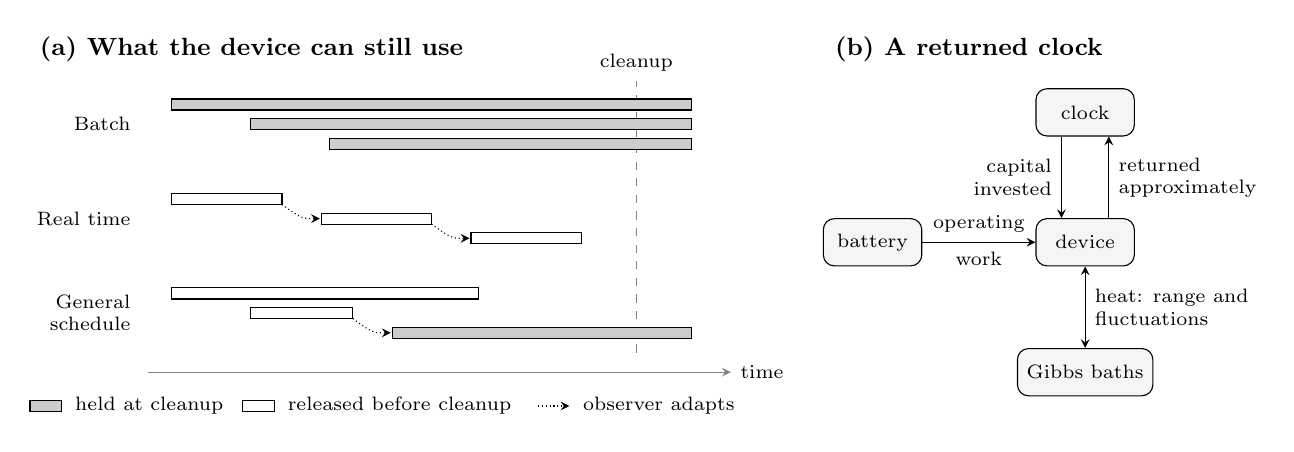
\begin{tikzpicture}[>=stealth, font=\scriptsize, box/.style={draw, rounded corners, minimum width=1.25cm, minimum height=0.6cm, fill=gray!8}]
  \node[font=\small\bfseries, anchor=west] at (-1.5,3.35) {(a) What the device can still use};
  \draw[dashed, gray] (6.2,-0.5) -- (6.2,2.95) node[above, black] {cleanup};
  \draw[->, gray] (0,-0.75) -- (7.4,-0.75) node[right, black] {time};
  \node[anchor=east] at (-0.1,2.4) {Batch};
  \node[anchor=east] at (-0.1,1.2) {Real time};
  \node[anchor=east, align=right] at (-0.1,0) {General\\schedule};
  \foreach \a/\y in {0.3/2.65, 1.3/2.4, 2.3/2.15} {\draw[fill=gray!40] (\a,\y-0.07) rectangle (6.9,\y+0.07);}
  \foreach \a/\b/\y in {0.3/1.7/1.45, 2.2/3.6/1.2, 4.1/5.5/0.95} {\draw[fill=white] (\a,\y-0.07) rectangle (\b,\y+0.07);}
  \draw[->, densely dotted] (1.7,1.38) .. controls (1.95,1.2) .. (2.18,1.2);
  \draw[->, densely dotted] (3.6,1.13) .. controls (3.85,0.95) .. (4.08,0.95);
  \draw[fill=white] (0.3,0.18) rectangle (4.2,0.32);
  \draw[fill=white] (1.3,-0.07) rectangle (2.6,0.07);
  \draw[fill=gray!40] (3.1,-0.32) rectangle (6.9,-0.18);
  \draw[->, densely dotted] (2.6,-0.07) .. controls (2.85,-0.25) .. (3.08,-0.25);
  \draw[fill=gray!40] (-1.5,-1.25) rectangle (-1.1,-1.11); \node[anchor=west] at (-1.05,-1.18) {held at cleanup};
  \draw[fill=white] (1.2,-1.25) rectangle (1.6,-1.11); \node[anchor=west] at (1.65,-1.18) {released before cleanup};
  \draw[->, densely dotted] (4.95,-1.18) -- (5.35,-1.18); \node[anchor=west] at (5.4,-1.18) {observer adapts};
  \begin{scope}[xshift=9.2cm]
  \node[font=\small\bfseries, anchor=west] at (-0.6,3.35) {(b) A returned clock};
  \node[box] (bat) at (0,0.9) {battery};
  \node[box] (dev) at (2.7,0.9) {device};
  \node[box] (clk) at (2.7,2.55) {clock};
  \node[box, align=center] (bath) at (2.7,-0.75) {Gibbs baths};
  \draw[->] (bat) -- node[above] {operating} node[below] {work} (dev);
  \draw[->] ([xshift=-0.3cm]clk.south) -- node[left, align=right] {capital\\invested} ([xshift=-0.3cm]dev.north);
  \draw[<-] ([xshift=0.3cm]clk.south) -- node[right, align=left] {returned\\approximately} ([xshift=0.3cm]dev.north);
  \draw[<->] (dev) -- node[right, align=left] {heat: range and\\fluctuations} (bath);
  \end{scope}
\end{tikzpicture}
\caption{(a) Three schedules for three uses. Each bar is a visit: the device can act on a carrier from its arrival, the left end, to its release, the right end. Shaded carriers are still held when the device cleans up and can serve as side information; for carriers released earlier, whatever the device's record shares with them is stranded. Dotted arrows mark the observer choosing a later input after seeing an earlier output. In the general schedule visits overlap and releases need not follow the order of arrivals. (b) A clock lent to the device for a target that is not time-covariant keeps separate ledgers: the operating work, given by the schedule law; the invested capital, which must come back approximately; and the range and fluctuations of the heat exchanged with the baths, which for a gate grow with the number of uses~\cite{KeepingTime}.}
\label{fig:schedules}
\end{figure}

\paragraph{Order, not speed.} Finite-time thermodynamics charges for speed: its excess work vanishes when a process runs slowly enough~\cite{SalamonBerry83,Crooks07,Proesmans20}. The costs here do not. All our rates allow devices of any size and any running time. A real-time Werner--Holevo device pays $\kB T\ln3$ per use however slowly it runs~\cite{ImmediateDelivery,SaveWork}, while a device that may wait pays essentially nothing, since the channel's thermodynamic capacity is zero~\cite{FBB21}. Thermodynamics therefore charges for time twice: once for speed, which patience removes, and once for order, which it does not. For classical information engines, costs that survive slow operation because processing goes step by step are known: the modularity dissipation of information ratchets~\cite{BMC18}, which Loomis and Crutchfield trace to temporal locality~\cite{LoomisCrutchfield20}, and the online cost of agents~\cite{Thompson25}. Here the price is forced by the release schedule for every implementation, and for channels it is purely quantum. The resource is not elapsed time. It is the capability that must remain available after access to an earlier output has been irreversibly surrendered.

\paragraph{Results.}
\begin{itemize}[leftmargin=*]
\item \emph{One law} (Section~\ref{sec:law}). For every finite schedule of arrivals, releases, retention and loans of carriers the observer owns, each returned with the Hamiltonian it arrived with, the work rate is a single entropy-plus-energy functional. Batch, real time, delayed release, interactive processes and clocks are special schedules (Section~\ref{sec:table}).
\item \emph{The companion results as schedules} (Sections~\ref{sec:waiting} and~\ref{sec:clock}). Waiting saves work only through side information and only for quantum channels~\cite{SaveWork}, and a returned clock has an exact batch price, under which a process and its time reverse can cost different amounts~\cite{KeepingTime}. New here: in entanglement cost, one more step of delay is worth exactly the questions it moves to the accessible side of a release; which carriers to hold costs a rank, and choosing them well is NP-hard; and the free processes of the three models are assembled into a strict ladder (Table~\ref{tab:ladder}).
\item \emph{Holding is decidable, releasing is not} (Section~\ref{sec:computability}). Whether a channel is free is a linear question when outputs may be held and undecidable when they must be released; the undecidability is thermodynamic, not chronological.
\item \emph{Beyond thermodynamics} (Section~\ref{sec:beyond}). Time order carries a per-use price in entanglement and coherence theory as well. In these examples the price is the formation cost of one common causal realization, which extends the entanglement cost of steering assemblages~\cite{Cope21}; whether this holds in general is open. In these delayed-choice examples one retained qubit is the common requirement, but there is no single exchange rate between theories.
\item \emph{Speed, order and a measurement} (Section~\ref{sec:measure}). With a finite thermal interface the two prices interact, and the order cost is the difference between the slow-limit intercepts of two schedules.
\end{itemize}

\paragraph{Two layers.} The mechanism is not specific to heat; what thermodynamics adds is the form of the price and its complexity. The free energy relative to the Gibbs state splits across a release as
\[
D(\rho_{CO}\|\gamma_C\otimes\gamma_O)=D(\rho_C\|\gamma_C)+D(\rho_O\|\gamma_O)+I(C{:}O),
\]
so at a fixed state the price of releasing $O$ from a device $C$ is a mutual information. Optimized over inputs, the surcharge is a difference of two maxima rather than the largest mutual information, because the two maxima can sit at different inputs (Section~\ref{sec:waiting}). For classical computation this is the modularity dissipation of Boyd, Mandal and Crutchfield, the free energy of correlations lost to local control~\cite{BMC18}; here the cut is a release in time. And the set of channels that cost nothing in real time is undecidable, while its batch counterpart, and every analogue we know outside thermodynamics, is decidable.

% =====================================================================
\section{Schedules and the law}\label{sec:law}

\paragraph{The device.} Entropies are in bits, except in Appendix~\ref{app:schedules}, which uses nats. We use the model of~\cite[Sec.~2]{SaveWork}. A device consists of a controller, a mechanical battery and Gibbs reservoirs at inverse temperature $\beta$, all declared in advance. Every operation is a unitary that conserves the total energy of the systems it acts on; there is no external coherence and no Gibbs-preserving map supplied as a black box. The controller returns approximately: its final joint state with everything else is close to its initial state tensored with the rest, and its actual mean energy and its actual entropy each change by $o(n)$. Trace-distance closeness alone would not suffice, since a broad register shifted down by $n$ levels is close to itself yet supplies $n$ quanta of work. Work is the battery's mean energy loss; the battery's entropy changes by $o(n)$, and work is \emph{deterministic} when the battery starts in an energy eigenstate, ends in a fixed energy level with probability tending to one, and its mean absolute energy deviation from that level is $o(n)$. The battery is \emph{stationary} if it starts in a state that commutes with its Hamiltonian; a battery in a broad superposition of energy levels would itself be a clock~\cite{SaveWork}.

\begin{definition}[Schedule]\label{def:schedule}
A schedule $S$ is a finite, ordered list of arrival and release events. A visit $v$ brings a carrier $P_v$ with Hamiltonian $H_v$ into the device at its arrival and returns the same carrier, with the same Hamiltonian, at its release. Visits of the same carrier cannot overlap; visits of different carriers may overlap, and releases may come in any order. The device can act on a carrier only during its visit. A later loan of a carrier that the observer owns is a new visit, and its state may be correlated with everything the observer holds. The observer supplies the carriers and may choose them adaptively, using only outputs already released, its own memory and its quantum references; every receipt or message the observer sees is written on a carrier the observer has supplied, and its delivery is that carrier's release.
\end{definition}

Batch operation is the schedule in which every input arrives before any output is released; real time is the schedule in which input $t+1$ arrives only after output $t$ has left; a process with memory interleaves the two.

\begin{definition}[The schedule functional]
A \emph{private extension} of a target strategy $T$ on $S$ consists of an initial device state $\tau$, an inert purification $F$ of it that is never acted on, and unitaries on the device and the carriers present, following $S$, whose marginal strategy is within $\varepsilon$ of $T$ in the strategy distance, the largest trace distance over adaptive testers. These unitaries need not conserve energy; the extension is a mathematical object. For a tester $t$, let $Z$ be everything the tester holds at the end, including its references and all released carriers, and let $E_t=\sum_v[\Tr H_v\rho_{v,\mathrm{release}}-\Tr H_v\rho_{v,\mathrm{arrival}}]$ be the energy handed over. Set
\[
k_{S,\varepsilon}(T)=\inf_{\text{private extensions}}\ \sup_t\Bigl[\tfrac{\ln2}\beta S(Z|F)_t+E_t\Bigr],
\]
and let $K_\beta^S(T)=\beta\,\bar k^S(T)/\ln2$, where $\bar k^S(T)=\inf_{\varepsilon_n\to0}\limsup_n k_{S_n,\varepsilon_n}(T_n)/n$ is the regularized rate along the block schedules $S_n$. As a check of the normalization, resetting a maximally mixed bit with zero Hamiltonian gives $k=\kB T\ln2$.
\end{definition}

By global purity, $S(Z|F)$ is the entropy the extension adds to its own record: the device cannot read $F$, and the same tester supplies both the entropy and the energy term. Table~\ref{tab:contract} collects the contract under which the law holds.

\begin{table}[tbp]
\centering
\small
\begin{tabular}{@{}>{\raggedright\arraybackslash}p{2.6cm}>{\raggedright\arraybackslash}p{12.2cm}@{}}
\toprule
Part of the contract & What it requires\\
\midrule
Target & A finite strategy on a specified schedule, such as a channel, a process or a delayed release, required of every observer, including inputs entangled with references the observer keeps.\\
Access & Inputs arrive and outputs are released as the schedule says; the observer chooses later inputs using released outputs, its memory and its references.\\
Ports & Each visit returns the same carrier with the Hamiltonian it arrived with. New or retired carriers need an inventory term, and changed Hamiltonians need a physical switch (Section~\ref{sec:law}).\\
Free dynamics & Unitaries that conserve the energy of the systems they act on, and Gibbs reservoirs at one temperature, declared in advance.\\
Controller & Returns approximately: its joint state with everything else ends close to its initial state tensored with the rest, and its actual mean energy and entropy each change by $o(n)$. Its startup capital is declared and may grow with $n$; it is not part of the rate.\\
Battery & Mechanical, with entropy change $o(n)$. Deterministic work: it starts in an energy eigenstate and ends in a fixed level with probability tending to one, with mean absolute deviation $o(n)$.\\
Limit & The error over the whole block of $n$ uses tends to zero, and the rate is per use as $n\to\infty$. Devices may have any size and running time. A rate of zero does not mean that a finite device runs at zero cost.\\
\bottomrule
\end{tabular}
\caption{The operational contract of Theorem~\ref{thm:law}. The rows on exact return and zero error in Table~\ref{tab:corollaries} lie outside it. Appendix~\ref{app:schedules} states the contract in full.}\label{tab:contract}
\end{table}

\begin{theorem}[Work law for schedules]\label{thm:law}
Let $S_n$ be the schedule of a block of $n$ uses, with the order of events across uses specified, in which each visit returns the same carrier with an unchanged Hamiltonian. The optimal rate of deterministic work for a device that returns its controller approximately is
\[
W^S=\frac{\ln2}{\beta}\,K_\beta^S.
\]
The lower bound holds for every implementation; the rate is attained using the finite-source and phase modules of~\cite[App.~E]{Answering}. Appendix~\ref{app:schedules} states the full contract, including the battery's absolute energy deviation. Resources that start correlated with the controller and must be returned in a prescribed joint state are not covered.
\end{theorem}

The lower bound is the accounting identity of~\cite{SaveWork} accumulated along the schedule: each release removes from the device's reach whatever its record shares with the released carrier. On a rare branch, the construction keeps a record of the observer's strategy, read from the arriving carriers; a positive correction, obtained by duality, is then paid as heat, and the required initial state is formed with the modules of~\cite[App.~E]{Answering}. Windows that collect a bundle of carriers and release it without feedback reduce exactly to the interleaved processes of~\cite{Answering}. General schedules, with overlapping visits, out-of-order releases and correlated re-entry, need the record to be kept on the actual carriers, with a positive dual correction at the end (Appendices~\ref{app:law} and~\ref{app:schedules}). The record is coherent: the construction neither identifies the observer by tomography nor measures the ordinary history. Its purpose is to make the unused part of a worst-case work budget a positive effect on systems the device still holds (Figure~\ref{fig:ledger}).

\begin{figure}[t]
\centering
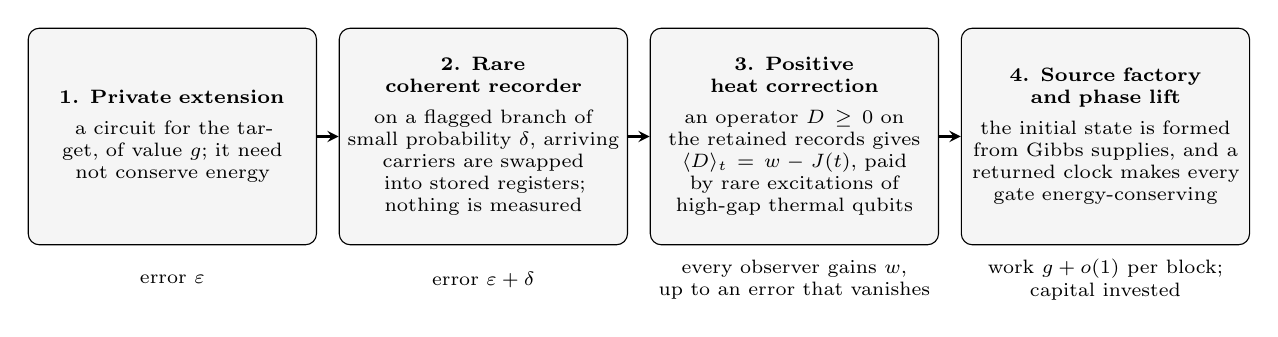
\begin{tikzpicture}[>=stealth, font=\scriptsize, stage/.style={draw, rounded corners, fill=gray!8, text width=3.45cm, align=center, minimum height=2.75cm, inner sep=3pt, anchor=north}]
  \node[stage] (s1) at (0,0) {\textbf{1. Private extension}\\[3pt] a circuit for the target, of value $g$; it need not conserve energy};
  \node[stage] (s2) at (3.95,0) {\textbf{2. Rare}\\\textbf{coherent recorder}\\[3pt] on a flagged branch of small probability $\delta$, arriving carriers are swapped into stored registers; nothing is measured};
  \node[stage] (s3) at (7.9,0) {\textbf{3. Positive heat correction}\\[3pt] an operator $D\ge0$ on the retained records gives $\langle D\rangle_t=w-J(t)$, paid by rare excitations of high-gap thermal qubits};
  \node[stage] (s4) at (11.85,0) {\textbf{4. Source factory and phase lift}\\[3pt] the initial state is formed from Gibbs supplies, and a returned clock makes every gate energy-conserving};
  \draw[->, thick] (s1) -- (s2); \draw[->, thick] (s2) -- (s3); \draw[->, thick] (s3) -- (s4);
  \node[align=center] at (0,-3.2) {error $\varepsilon$};
  \node[align=center] at (3.95,-3.2) {error $\varepsilon+\delta$};
  \node[align=center] at (7.9,-3.2) {every observer gains $w$,\\up to an error that vanishes};
  \node[align=center] at (11.85,-3.2) {work $g+o(1)$ per block;\\capital invested};
\end{tikzpicture}
\caption{The construction behind the upper bound of Theorem~\ref{thm:law}, read as a ledger (Appendix~\ref{app:schedules}). The record in stage~2 is coherent: no history is measured or postselected, and the rare branch adds only a small error. Stage~3 makes the unused part of the worst-case budget, $w-J(t)$ for the observer $t$, a positive effect on systems the device still holds, so every observer is charged the same work. Stage~4 is the finite-source and phase module of~\cite[App.~E]{Answering}; its capital can be enormous, but it is invested, not consumed, and comes back with the controller.}
\label{fig:ledger}
\end{figure}

Three remarks fix the scope.

\paragraph{New and retired carriers.} A schedule that delivers new output carriers, or retires inputs, needs the inventory term $(\sum_{\mathrm{new}}\ln Z_O-\sum_{\mathrm{retired}}\ln Z_I)/\beta$ in the functional; without it even the preparation of a thermal state is mispriced. The lower bound with this term holds for every schedule, since the accounting identity changes the stock's partition function by exactly this amount. In batch, for a time-covariant channel $\Phi_{A\to B}$, the corrected formula is a theorem: the capacity theorem~\cite[Thm.~7.1]{FBB21}, applied to the time-covariant channel $X_{AB}\mapsto\gamma_A\otimes\Phi(\Tr_BX_{AB})$ on the fixed composite system $AB$ with Hamiltonian $H_A+H_B$, attains it, because the capacity of that channel is $\sup_\sigma[D(\Phi(\sigma)\|\gamma_B)-D(\sigma\|\gamma_A)]$. For general schedules with new or retired carriers, a matching construction depends on a source-formation step that we do not prove here.

\paragraph{Return rules.} Return rules cannot be arbitrary: a controller that returns only in trace distance can supply extensive work, so the contract must also refund actual energy and actual entropy; neither alone suffices, and since the lower bound sees the controller only through $\Delta E_C-(\ln2/\beta)\Delta S_C$, we require each to change by $o(n)$.

\paragraph{Changing Hamiltonians.} Changes of Hamiltonian are not free relabellings: after a release, a retained switch cannot be reset between modes that assign the released system different energy gaps using only energy-conserving operations on what the device keeps, so a schedule that changes Hamiltonians must count the switch as a physical system.

% =====================================================================
\section{One functional, many schedules}\label{sec:table}

Most rows of Table~\ref{tab:corollaries} are Theorem~\ref{thm:law} evaluated on one schedule; the rows on exact return, on zero error and on the clock's capital lie outside its hypotheses and are listed for comparison. For a clock returned in batch, Theorem~\ref{thm:batchlaw} gives the same optimal rate in single-letter form, $B(\Phi)$, so the two agree.

\begin{table}[tbp]
\centering
\small
\begin{tabular}{>{\raggedright\arraybackslash}p{4.0cm}>{\raggedright\arraybackslash}p{3.2cm}>{\raggedright\arraybackslash}p{6.2cm}}
\toprule
Result & Schedule & Value\\
\midrule
Landauer erasure~\cite{Landauer61} & any & $\kB T\ln2$ per bit, degenerate levels\\
Batch capacity, covariant channels & hold all outputs & the capacity of~\cite{FBB21}\\
Real-time channels & release each output & $\kB T\ln2\,\Trt(\Phi)$; equal to the capacity for classical channels~\cite{SaveWork}\\
Processes with memory & interleaved & $\kB T\ln2\,K_\beta(\mathcal P)$ for every finite process~\cite{Answering}\\
Order alone & two-step classical process & $\kB T\ln2\,[1-h_2(p)]$ per episode if released early, $0$ if held, with $p$ the bias of the process's coin~\cite{Answering}\\
Which carriers to hold & linear task, carriers $L$ released early & $\operatorname{rank}(F_L)\,\kB T\ln2$ per use; the best choice under a budget is NP-hard (Proposition~\ref{prop:rank})\\
Delayed channel & ground state first, $\Phi$ of the first input one slot later, second input discarded & $\Trt(\Phi)+\log_2\Tr e^{-\beta(H-E_0)}$ bits; the second term pays for discarding the second input~\cite{Answering}\\
Clock returned exactly & non-covariant target & impossible at any work, with a stationary battery~\cite{SaveWork}\\
Clock returned approximately & non-covariant target & real-time rate $\Trt$; capital, bath range and lottery for gates~\cite{SaveWork,KeepingTime}\\
Batch with a returned clock & hold all, clock returned & $B(\Phi)$; the capacity when $H-\Phi^*H\in\mathrm{span}\{A_i^*A_j\}$~\cite{KeepingTime}\\
$X$-dephasing & hold all, clock returned & $E/2$, as in real time; capacity $\beta^{-1}\ln\cosh(\beta E/2)$~\cite{KeepingTime}\\
Gibbs preservation & hold all, clock returned & a positive rate per use at zero capacity~\cite{KeepingTime}\\
Process vs.\ time reverse & hold all, clock returned & qutrit: $0.1547\,\kB T$ against $0$~\cite{KeepingTime}\\
Zero error, extreme channels & hold all & the full real-time rate~\cite{SaveWork}\\
\bottomrule
\end{tabular}
\caption{One functional, many schedules. Values are work per use unless marked per episode. $\Trt$, $K_\beta$ and the capacity $\mathcal T$ are in bits, to be multiplied by $\kB T\ln2$; $B(\Phi)$ and quantities written with $E$ are energies. The rows on exact return and on zero error lie outside the hypotheses of Theorem~\ref{thm:law} and are listed for comparison.}\label{tab:corollaries}
\end{table}

The real-time rate is $\Trt(\Phi)=\sup_\rho[S(\rho)-S(\Phi(\rho))+m_\rho+\beta\Tr H(\Phi(\rho)-\rho)/\ln2]$, where $m_\rho$ is the least mutual information any exact dilation must leave between the released output and what stays in the device; the thermodynamic capacity of Faist, Berta and Brand\~ao is the same expression with $m_\rho=0$~\cite{FBB19,FBB21,SaveWork}. For processes, $K_\beta$ is an entropy change plus an energy change measured against the same adaptive observer and minimized over implementations that respect the order in which outputs are due~\cite{Answering}. The batch quantity $B(\Phi)$ is defined in Section~\ref{sec:clock}.

% =====================================================================
\section{What waiting buys}\label{sec:waiting}

\paragraph{Side information.} Erasing a memory $M$ with quantum side information $O$, while leaving $O$ and its correlations with everything else intact, costs $\kB T\ln2\,S(M|O)$ per copy; del Rio et al.\ showed that this much work suffices, even when it is negative~\cite{delRio11}. Without the side information it costs $\kB T\ln2\,S(M)$, more by the mutual information $I(M{:}O)$. A batch device keeps its outputs as side information until it has cleaned up~\cite[Sec.~7]{FBB21}; a real-time device has already released them. At a fixed input $\rho$, the real-time integrand exceeds the batch one by $m_\rho$, the least such mutual information an implementation must leave, which can be smaller than any particular dilation suggests. For time-covariant channels the optimal batch rate in this thermal-operation model is the thermodynamic capacity $\mathcal T(\Phi)=\max_\rho c_\rho$, where $c_\rho=S(\rho)-S(\Phi(\rho))+\beta\Tr H(\Phi(\rho)-\rho)/\ln2$, so the surcharge between the optimal rates is $\Trt(\Phi)-\mathcal T(\Phi)=\max_\rho(c_\rho+m_\rho)-\max_\rho c_\rho$. It is not an optimum of $m_\rho$ alone, because the two maxima can sit at different inputs. The extra term $m_\rho$ is a correlation cost, input by input; the surcharge compares two optimized totals. For amplitude damping at $p=1/2$ and $\beta E=\ln2$ (Figure~\ref{fig:surcharge}), $m_\rho=0.918$ bits at the real-time optimum, while the surcharge is $0.585E-0.154E=0.431E$ per use, that is $0.431$ bits. For a general channel with a returned clock the batch endpoint is instead $B(\Phi)$ of Section~\ref{sec:clock}, and the saving from waiting is $\kB T\ln2\,\Trt(\Phi)-B(\Phi)$. The capacity gap remains a benchmark, but it need not be a saving available under that return contract: $X$-dephasing costs $E/2$ per use in both schedules, above its capacity. A classical channel can keep a copy of each output before releasing it, so it pays nothing extra, much as an information ratchet avoids modularity dissipation by keeping the correlations it would otherwise lose~\cite{BMC18}; a quantum channel cannot copy, and partial reset of a qubit pays a surcharge at every temperature~\cite{SaveWork}. Only quantum channels save work by waiting. Here a channel means repeated uses of one memoryless map: classical tasks with several steps can also save work by waiting, as Proposition~\ref{prop:rank} shows exactly. This concerns the channel, not the memory: for classical strategies, a quantum memory can lower the online cost~\cite{Thompson25}.

\begin{figure}[t]
\centering
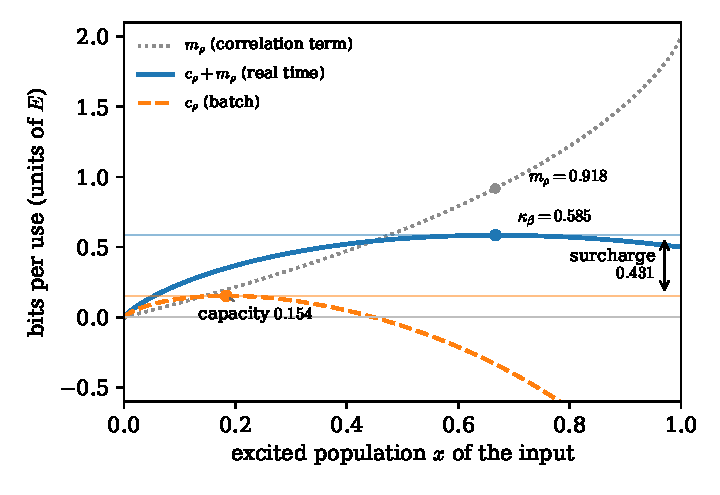
\includegraphics[width=0.62\linewidth]{fig-surcharge.pdf}
\caption{The surcharge is a difference of two maxima. Amplitude damping with $p=1/2$ at $\beta E=\ln2$, so that one bit costs $E$; inputs diagonal in the energy basis, with excited population $x$, attain both maxima. Dashed: the batch integrand $c_\rho=h(x)-h(x/2)-x/2$, whose maximum is the capacity, $0.154$, at $x\approx0.18$. Solid: the real-time integrand $c_\rho+m_\rho=h(x/2)-x/2$, whose maximum is $\Trt=0.585$, at $x=2/3$. Dotted: the correlation term $m_\rho=2h(x/2)-h(x)$. The surcharge, $0.431$, is neither $m_\rho$ at the real-time optimum, $0.918$, nor $m_\rho$ at the batch optimum, $0.197$.}
\label{fig:surcharge}
\end{figure}

\paragraph{Error.} For extreme channels, the batch saving requires nonzero error, even when that error vanishes with the block size.

\begin{proposition}[Zero error removes the saving for extreme channels~\cite{SaveWork}]
If a channel is extreme in the convex set of channels, every implementation with zero error, in batch or in real time, pays the real-time rate.
\end{proposition}

Extremality makes the branches of any exact implementation orthogonal~\cite{Choi75}, so the device's entropy rises by exactly the entropy of the complementary output on every input. For amplitude damping at $p=1/2$ and $\beta E=\ln2$, the real-time rate is $0.585\,E$ per use and the batch capacity $0.154\,E$~\cite{SaveWork}; the difference is available only to a device that tolerates some error.

\paragraph{Delay.} Let each output be released $b$ steps later than in real time. For independent delayed-choice episodes, in which a qubit is released and the question it must answer arrives $\ell_i$ steps later, the number of episodes that still require an early commitment is $\#\{i:\ell_i>b\}$, and under one-way communication from the party that answers, the entanglement cost is exactly this number (a question that arrives in the same step as the delayed release is taken to arrive first): each such episode is charged one ebit by the monogamy argument of Section~\ref{sec:beyond}, and every other episode is answered before its release at no cost. One more step of delay saves $\#\{i:\ell_i=b+1\}$: a step of delay is worth exactly the questions it moves to the accessible side of a release, and has no fixed exchange value. Under the strict real-time rule, where the next input arrives only after the last output has left, waiting longer does not move any question and buys nothing. For repeated uses of one channel, block constructions with exponentially small block errors reach the batch rate once the delay is of order $\log(n/\varepsilon)$, by running blocks of that length in batch and taking a union bound over blocks; the exact work--latency profile is open.

\paragraph{Which carriers to hold.} With several carriers in flight, a schedule can let some of them wait for a later input while others leave. For linear tasks the price of such a schedule is a rank, and the best choice of what to hold is a question about codes. For example, let the late output need the two parities $a_1\oplus a_2$ and $a_2\oplus a_3$, so that $F$ has rows $(1,1,0)$ and $(0,1,1)$. Releasing all three bits costs two bits. Holding any one of them still leaves released columns of rank two, so it saves nothing; holding any two leaves a single nonzero column and lowers the cost to one bit; holding all three makes it zero. A held bit helps only when it completes a late parity, not merely because it is one more bit of storage.

\begin{proposition}[Release rank]\label{prop:rank}
Let $F$ be an $\ell\times k$ binary matrix. A device receives $a\in\mathbb F_2^k$ on $k$ bit carriers with zero Hamiltonian. The carriers in a set $L$ must leave, unchanged, before a fresh $b\in\mathbb F_2^\ell$ arrives on $\ell$ further carriers; those in $R=\{1,\dots,k\}\setminus L$ may be held until then. In the end the device returns every first carrier unchanged and dephased, and the second carriers holding $b\oplus Fa$. Let $D$ be everything the device keeps, initially independent of the inputs, and let $F_L$ be the columns of $F$ in $L$.
\begin{enumerate}[label=(\alph*)]
\item For independent uniform $a$ and $b$, every exact implementation raises the entropy of $D$ by at least $\operatorname{rank}F_L$ bits, so, when its controller, battery and Gibbs reservoirs start independent, it dumps heat at least $[\operatorname{rank}F_L-\Delta S_C-\Delta S_W]\,\kB T\ln2$, with $\Delta S_C$ and $\Delta S_W$ the entropy changes of its controller and battery in bits. An energy-conserving implementation raises the entropy by exactly $\operatorname{rank}F_L$ and dumps heat $(1-q)\operatorname{rank}(F_L)\,\kB T\ln2$, where $q$, the probability that its battery misses its final level, can be made as small as desired.
\item If any $m$ carriers may be held, the least cost is $\operatorname{rank}F-\max\{r:d_r(\mathcal C)\le m\}$ bits, where $\mathcal C$ is the row space of $F$ and $d_r(\mathcal C)$, its $r$-th generalized Hamming weight, is the smallest support of an $r$-dimensional subcode~\cite{Wei91}. Holding $m$ carriers lowers the cost at all exactly when $\mathcal C$ has a nonzero word of weight at most $m$, which is NP-complete to decide~\cite{Vardy97}.
\end{enumerate}
\end{proposition}

Holding every carrier costs nothing, and holding one more carrier helps only when it completes a late parity, one that then depends on held carriers alone: the price $\operatorname{rank}F_L=\operatorname{rank}F-\dim\mathcal C(R)$ counts the independent parities of the released bits that the late output still needs, where $\mathcal C(R)$ is the set of late parities supported on held carriers. By part (b), the price of a schedule is a coding invariant of the task: its generalized Hamming weights, which Wei introduced for the wire-tap channel of type II~\cite{Wei91}. The proof is in Appendix~\ref{app:rank}.

% =====================================================================
\section{Returning a clock}\label{sec:clock}

A channel that is not time-covariant needs a phase reference. If the reference is finite-dimensional and must come back exactly, and the battery is stationary, no such channel can be run at any work cost: by the no-broadcasting theorem for asymmetry, a bounded reference used to implement an operation that is not covariant is necessarily degraded~\cite{MarvianSpekkens19,LostaglioMuller19}; if it need only come back approximately, every channel runs in real time at the rate $\Trt$~\cite{SaveWork}. For a gate the reference then pays in other currencies: capital at least of order $n/(\varepsilon+\eta)$, baths whose energy range grows at least like $n/\sqrt\varepsilon$, and an energy that returns only as a lottery~\cite{KeepingTime}. The capital has the scaling of the reference-size laws of Chiribella, Yang and Renner and of Tajima, Shiraishi and Saito~\cite{ChiribellaYangRenner21,TSS20}. Channels that are not gates can need far less: a Gibbs-preserving qubit channel that is not time-covariant runs in batch at zero work with a clock whose spread grows like $\sqrt n$~\cite{KeepingTime}.

In batch the returned clock has an exact price. Let $\Psi$ be a complementary channel, $D=\Phi^*(H)-H$ and
\[
B(\Phi)=\max\bigl\{\Tr\rho D+\kB T\ln2\,[S(\sigma)-S(\Phi(\sigma))]\;:\;\Psi(\rho)=\Psi(\sigma)\bigr\}.
\]

\begin{theorem}[The batch law with a returned clock~\cite{KeepingTime}]\label{thm:batchlaw}
With a battery that starts in an energy eigenstate and a controller that returns approximately, all of it and not only the clock, the optimal batch work per use of every finite channel is $B(\Phi)$, attained with deterministic work. It equals $\kB T\ln2\,\mathcal T(\Phi)$, the thermodynamic capacity in energy units, whenever $D$ lies in the span of the products $A_i^*A_j$ of Kraus operators, and a Gibbs-preserving channel is free exactly when it does.
\end{theorem}

Two inputs can be charged separately, one for energy and one for entropy, exactly when the environment cannot tell them apart. When the environment can carry the energy change, input by input on average, the clock never has to absorb an energy that depends on the input, and the capacity is reached. A returned clock can supply phase, but it cannot provide net extensive energy: for every observer its actual mean energy change must be sublinear. It can still make large loans that depend on the branch, as long as their mean is refunded. Otherwise the remainder is paid. Qubit dephasing in the $X$ basis costs $E/2$ per use in batch, exactly its real-time cost and above its capacity; some Gibbs-preserving channels, of capacity zero, cost work of order $n$; and every Gibbs-preserving qubit channel is free in batch with a returned clock~\cite{KeepingTime}. The span of the products $A_i^*A_j$ is the non-commutative confusability graph of Duan, Severini and Winter~\cite{DSW13}. The same condition separates small clocks from large ones. When $D$ lies outside the span, the channel's time evolution, whose generator is exactly $D$, can be estimated at the Heisenberg limit~\cite{ZhouJiang21}, so the channel can read its own clock to within $1/n$, and no clock whose spread grows more slowly than $n$ can run it reliably, at any work~\cite{KeepingTime}.

\begin{table}[tbp]
\centering
\small
\begin{tabular}{>{\raggedright\arraybackslash}p{4.6cm}>{\raggedright\arraybackslash}p{6.6cm}l}
\toprule
Schedule and clock & Processes that cost nothing & Decidable\\
\midrule
Batch, Gibbs-preserving maps free~\cite{FBB21} & Gibbs-preserving channels & yes\\
Batch, clock returned & Gibbs-preserving, with $H-\Phi^*H\in\mathrm{span}\{A_i^*A_j\}$ & yes\\
Real time & limits of thermal operations~\cite{SaveWork} & no\\
\bottomrule
\end{tabular}
\caption{The free channels shrink as the operational model tightens: Gibbs-preserving maps taken as free operations, thermal operations with a returned clock in batch, and thermal operations in real time. Each inclusion is strict: a Gibbs-preserving qutrit separates the first two rows~\cite{KeepingTime}, the Werner--Holevo channel, which is not factorizable~\cite{HaagerupMusat11}, the last two.}\label{tab:ladder}
\end{table}

\paragraph{A process and its time reverse.} For a Gibbs-preserving channel, the reverse process of quantum fluctuation theorems~\cite{Crooks08,KwonKim19} is its Petz map $\Phi^\sharp(\sigma)=\gamma^{1/2}\Phi^*(\gamma^{-1/2}\sigma\gamma^{-1/2})\gamma^{1/2}$. Thermal operations are closed under this reversal. With a returned clock, the criterion of Theorem~\ref{thm:batchlaw} is not: on a qutrit there is a Gibbs-preserving channel that costs $0.1547\,\kB T$ per use while its reverse costs nothing~\cite{KeepingTime}. Which direction is free is decided by two linear tests on the Kraus operators. The asymmetry is not generic: channels of full Kraus rank pass both tests, so any fixed amount of full-rank thermal noise removes it, and separated pairs lie on the boundary of the channel set. For a finite device the threshold is set by the horizon: noise removes the asymmetry only when the expected number of noisy uses grows without bound, so noise per use small compared with the inverse of the number of uses leaves the full cost in place~\cite{KeepingTime}. In coherence the same pair is already asymmetric: by the theorem of Tajima and Takagi the forward channel needs coherence that diverges as the error vanishes, while its reverse creates coherence at finite cost~\cite{TajimaTakagi25}. With a returned clock the asymmetry appears in work. It is an implementation asymmetry created by the obligation to return the clock. It does not violate any fluctuation theorem, and it is not carried by the clock, whose entropy changes by $o(n)$.

% =====================================================================
\section{Holding is decidable, releasing is not}\label{sec:computability}

In batch, whether a channel costs nothing is a linear condition: Gibbs preservation, and with a returned clock the span condition of Theorem~\ref{thm:batchlaw}. For a channel given exactly, for example with algebraic entries, the batch cost with a returned clock, $B(\Phi)$, is a finite-dimensional optimization that can be computed to any precision; unlike the capacity, it is not continuous in the channel, so it cannot be estimated uniformly from approximate data. In real time, a channel costs nothing exactly when it is a limit of thermal operations, and no algorithm decides membership, even in a fixed dimension~\cite{SaveWork}, extending the zero-Hamiltonian result of~\cite{Flagship}. Choosing what to hold is hard in a different way: for the linear tasks of Proposition~\ref{prop:rank} the cost of each choice is a rank, computable in polynomial time, but deciding whether holding $m$ carriers lowers it at all is NP-complete.

The source of the undecidability is the absence of a computable bound on the size of the noncommutative dilations that witness membership. It is present already at zero Hamiltonian, where the question becomes whether a channel is a limit of finitely factorizable ones~\cite{Memory}, so Gibbs weights are not essential. It is also not a consequence of time order alone. Under local operations and classical communication, a channel is free in batch exactly when it is entanglement-breaking~\cite{HSR03},~\cite[Cor.~18]{BBCW13}, and so also in real time; this is a semialgebraic condition, decidable by quantifier elimination. Under one-way communication from the party that answers, a delayed-choice task is free in real time exactly when its assemblage has a local-hidden-state model, the free assemblages of the resource theory of steering~\cite{GallegoAolita15}; this is a semidefinite condition~\cite{CavalcantiSkrzypczyk17}. Outside that set, squashed entanglement is bounded below by a constant times the squared distance to the separable states in a one-way LOCC norm, with no dependence on dimension~\cite{BCY11}, so the rate is positive. Under incoherent operations a delayed-choice task is free exactly when its conditional states are diagonal. Unbounded free ancillas are not enough to make freeness undecidable. Among the theories treated here, thermodynamics is the one in which releasing in time makes the zero set uncomputable.

What the results show is operational. Being able to describe every event at once does not mean being able to act on every event at once. The difference has a price, and in thermodynamics whether that price is zero cannot be computed.

% =====================================================================
\section{Beyond thermodynamics}\label{sec:beyond}

The same mechanism appears wherever a released system must stay correlated with what the device keeps. Its sharpest form is a statement about quantum mechanics alone, best seen on one task.

\paragraph{The delayed-choice task.} The task has two outputs, a qubit $B$ and a classical bit $a$. The observer supplies a question $x$, which chooses one of two bases, and the device must return a uniformly random answer $a$ such that, given $x$ and $a$, the qubit $B$ is the corresponding basis state; for the BB84 task the bases are the computational and Hadamard bases. In batch the question arrives before $B$ is released. In real time it arrives afterwards, and the device never touches $B$ again. A Bell pair realizes the real-time task: release one half, and measure the retained half in the requested basis.

\begin{lemma}[Release lemma]\label{lem:release}
Suppose a qubit $B$ is released, and afterwards a memory $M$, which holds everything the device keeps at the release, must produce an answer $a$ such that, for either of two questions $x$ chosen after the release, the conditional states of $B$ are pure in a basis that depends on $x$. If the two bases do not commute, every exact realization has $-S(B|M)=1$. If each mismatch probability is at most $\varepsilon$, in particular at strategy error $\varepsilon$, then $-S(B|M)\ge1-g\bigl(\sqrt\varepsilon\,(1+2/\sin2\theta)\bigr)$ with $g(d)=2d+(1+d)\,h_2\bigl(d/(1+d)\bigr)$, where $\theta$ is the angle between the bases, independently of the dimension of $M$.
\end{lemma}

The exact statement is closely related to known results. The assemblages of the two questions are extremal for every nonzero angle, and Cope showed that every state realizing an extremal assemblage has entanglement of formation equal to the entropy of its reduced state, here one ebit~\cite[Thm.~1]{Cope21}; for the BB84 pair it also follows from one-sided self-testing of the ebit~\cite{SupicHoban16}, and the uncertainty relation with quantum memory gives $-S(B|M)\ge1-2h_2(\varepsilon)$~\cite{BCCRR10}. What the lemma adds is the form, a statement about whatever memory outlives a release, usable in every resource theory, and a robust bound that does not depend on the dimension of $M$.

Each resource theory converts $-S(B|M)$ into its own currency.
\begin{itemize}[leftmargin=*]
\item \emph{Entanglement under one-way communication from the party that answers to the party that releases.} For the delayed-choice BB84 task, holding the qubit costs nothing, while releasing it first costs exactly one ebit per use, extensively. The uncertainty relation with quantum memory~\cite{BCCRR10}, with Fano's inequality, gives $-S(B|M)\ge1-2h_2(\varepsilon)$; squashed entanglement~\cite{ChristandlWinter04} is at least $-S(B|M)$, by strong subadditivity; and its monogamy~\cite[Thm.~8]{KoashiWinter04} charges every release, so $n$ uses need $n[1-2h_2(\varepsilon)]$ ebits. By the release lemma the rate is the same for every tilt $\theta\in(0,\pi/2)$. Two-way communication removes the cost, because the releasing party can keep the partner of $B$ and report the answer.
\item \emph{Coherence under incoherent operations}~\cite{BCP14,WinterYang16}. For the delayed choice between the computational basis and a basis tilted by $\theta$, real time costs one coherent bit per use and batch costs $h_2(\sin^2\theta)$, the coherence cost~\cite{WinterYang16} of the tilted basis states, so the surcharge is $1-h_2(\sin^2\theta)$, $0.399$ at $\theta=\pi/8$. The surcharge approaches one bit as $\theta\to0$: for every fixed $\theta>0$ the real-time cost at vanishing error stays one coherent bit, while the batch cost $h_2(\sin^2\theta)$ tends to zero. It vanishes for mutually unbiased bases. A two-step process built from a CNOT and a dephasing of the first output in the $X$ basis, which is a free mixture of $I$ and $X$, costs nothing in batch and one coherent bit per episode in real time; $N$ episodes at error $\varepsilon$ consume at least $N[1-h_2(\varepsilon)]$ coherent bits net (Appendix~\ref{app:numbers}).
\end{itemize}
Pure memory, disposal and reset are free in both theories. In real time the answering party's messages reach the releasing party only after $B$ has left, so in these examples the real-time entanglement cost is the entanglement cost of the task's steering assemblage, which Cope defined~\cite{Cope21}. In the resource theory of steering, communication may run only from the party that holds the steered system, since communication towards it could create steering~\cite{GallegoAolita15}. Here it runs towards that party: in batch this is what makes the task free, and in real time the release order is what keeps it from creating steering. What is new is this comparison with batch, the surcharge for releasing rather than holding the same process. A per-use timing cost does not need forgetting to be priced; it needs only that the cheapest global implementation cannot be split, at the same cost, into stages that respect the release order.

\paragraph{Towards a general law.} In the examples above, the gross cost of a schedule is the smoothed regularized formation cost of one common source together with a free causal decoder, and the time-order surcharge is the difference between its real-time and batch values. We expect the same under general formation hypotheses, for instance for one-way communication whenever all released outputs leave before the first question; we do not state or prove them here. For a single release this extends the entanglement cost of steering assemblages~\cite{Cope21}. The smoothing matters: the entanglement of formation of an assemblage is not continuous, and Cope expects its plain regularization to differ from the cost~\cite{Cope21}. Removing the smoothing, crediting returned resources and factorizing interleaved releases remain open. Three quantities must be kept apart: consumption, a rate; working capital, the largest running deficit, which can be refilled by resources that arrive later; and sublinear irreversible overhead. The naive statement that the surcharge is the correlation forced across the release cut fails: in the tilted coherence task the forced correlation is one full bit, while the surcharge is $1-h_2(\sin^2\theta)$, because part of the correlation is later delivered to the observer as the output it asked for. That part must be credited.

\paragraph{No single currency.} The delayed-choice task certifies exactly one qubit of necessary quantum retention: a classical record across the cut, an entanglement-breaking memory in the sense of~\cite{RBL18}, cannot realize it, since $S(B|J)\ge0$ for classical $J$, and $-S(B|M)\le\log_2\dim M$ forces a qubit. This requirement is the same in every theory. Its price is not (Table~\ref{tab:currency}).

\begin{table}[tbp]
\centering
\small
\begin{tabular}{lccc}
\toprule
Theory & Real time & Batch & Order price\\
\midrule
Thermodynamics at zero Hamiltonian & $2\,\kB T\ln2$ & $\kB T\ln2$ & $\kB T\ln2$\\
Entanglement, one-way communication & $1$ ebit & $0$ & $1$ ebit\\
Coherence, incoherent operations & $1$ & $1$ & $0$\\
Magic, stabilizer operations & $0$ & $0$ & $0$\\
\bottomrule
\end{tabular}
\caption{The delayed-choice BB84 task in four resource theories. Coherence is counted in coherent bits; under stabilizer operations a Bell pair and Pauli measurements are free, so the task costs nothing in either schedule.}\label{tab:currency}
\end{table}

In the thermodynamic row the output registers are taken from the reservoir, so no blank register is free, and the setting register is read-only and returned; with free blank registers both thermodynamic entries fall by $2\,\kB T\ln2$, so that batch then extracts $\kB T\ln2$, and the order price is unchanged (Appendix~\ref{app:numbers}). In thermodynamics the Bell pair that realizes the task in real time is worth two bits of work; one bit is delivered to the observer as the output, and one is the price of order. The order prices are not proportional across tasks. In entanglement theory the BB84 task and the tilted task both carry an order price of one ebit; in coherence theory their order prices are $0$ and $0.399$. With rows for entanglement and coherence and columns for the BB84 and tilted tasks, the order prices form the matrix
\[
\begin{pmatrix}1&1\\0&0.399\end{pmatrix},
\]
which has rank two, so no amount of order per task multiplied by an exchange rate per theory reproduces it. Even an ordering of tasks by amount of order fails: the BB84 task has order price $1$ in entanglement theory and $0$ in coherence theory, while the CNOT process above, with its first slot at one party and its second at another, has order price $0$ in entanglement theory, since the first party can measure in the $X$ basis and tell the second which phase to apply, and $1$ in coherence theory. What these examples share is the requirement, one retained Bell pair. When the answering measurement is free, as in every row of the table, real time pays that Bell pair's price in the theory, and the order price is that price minus what the task would cost in batch. What replaces a currency is a budget region for each scheduled process, consumption, capital, reference and returns, which each theory values differently.

\paragraph{Order cannot be manufactured.} Call a process classical-retention if it can be realized with only classical records kept across each release cut. For a single cut these are the entanglement-breaking channels, the free objects of the resource theory of quantum memories~\cite{RBL18}; for many cuts they are the processes with classical memory of the multi-time resource theories of Berk et al.~\cite{Berk21}. As in those theories, any contractive distance to them, the strategy-norm distance included, cannot increase under schedule-respecting adapters that themselves keep only classical records across release cuts~\cite[Thm.~1]{Berk21}, so order cannot be manufactured by such adapters. Adapters that keep quantum memory are not free in this sense: an adapter that receives both halves of a Bell pair at once, releases one and holds the other across the release turns that source into the BB84 task. The surcharge itself is monotone only under conversions that preserve batch credits: a source that releases one half of a Bell pair early and delivers the other half late has surcharge $0$, and an adapter that keeps nothing, measuring the late half in the basis $x$, turns it into the BB84 task, whose surcharge is $1$.

% =====================================================================
\section{Speed, order and a measurement}\label{sec:measure}

\paragraph{Speed and order together.} Output deadlines alone impose no deadline on preparation or cleanup: a device can prepare its resources in advance, release its outputs on time and restore itself slowly afterwards. In our model the order cost is therefore pure order. A speed price appears only when the thermal interface is budgeted. Consider a collision model in which each thermal contact fully swaps one cell with a fresh Gibbs qubit. Let a device implement the target at error $\varepsilon$, and let it reset its cells along strokes of thermodynamic length $\ell_j$, each starting at excited population at most $1/2$, using $K_j$ contacts per stroke. Each contact is a step equilibration, and for a process carried out in $K$ such steps the dissipation is at least $\kB T\ell^2/(2K)$ to leading order in $1/K$, for thermodynamic length $\ell$~\cite{SalamonBerry83,Nulton85,Crooks07,ScandiPerarnauLlobet19,Abiuso20}. For these strokes the bound holds at every $K_j$, and summing over strokes gives
\[
W\ \ge\ W^{\mathrm{qs}}(\varepsilon)+\frac{\kB T}{2}\sum_j\frac{\ell_j^2}{K_j}\ \ge\ W^{\mathrm{qs}}(\varepsilon)+\kB T\,\frac{(\sum_j\ell_j)^2}{2K_{\mathrm{tot}}},
\]
where $W^{\mathrm{qs}}(\varepsilon)$ is the slow limit of the same device. For a device that attains its schedule's optimum it tends to $W^{\mathrm{qs}}_{\mathrm{batch}}+W_{\mathrm{order}}$ as $\varepsilon\to0$; any other device adds its own implementation overhead. For other strokes, including recoveries that extract work, the factor $1/2$ holds only to leading order in $1/K_j$; the factor $1/4$ holds exactly. When ordinary and order-forced resets, of total lengths $L_B$ and $L_O$, share $M$ contacts, the optimally scheduled work exceeds its value with separate interfaces by $\kB T\,L_BL_O/M+o(1/M)$, the cross term of $\kB T(L_B+L_O)^2/(2M)$. Order decides which resets must happen; speed charges for completing them in time. At a fixed number of contacts, driving the error to zero makes the work diverge, as finite resources forbid a perfect reset~\cite{ReebWolf14,Taranto23}, although only logarithmically for a single contact and far more slowly for several. Any finite law must therefore state its error.

\paragraph{A measurement.} Measure the work as a function of the thermal-contact budget $K$ for both schedules at the same certified error. Fit each curve by an intercept plus terms in $1/K$ and $1/K^2$, or by the exact finite-$K$ curve of the collision model, as tests of Landauer's principle extrapolate the work to slow operation~\cite{Berut12,Jun14}. The difference between the two slow-limit intercepts is the excess quasistatic work of the two implementations at the certified error. It equals the order surcharge only when both implementations attain their schedule optima; otherwise it also contains implementation overhead, and the finite certificates below give an unavoidable lower bound without any such optimality claim. The slopes carry speed, including the mixed term. Near a pure target the work approaches its $1/K$ law slowly: in the collision model above, for the amplitude-damping example below with a cell reset from its Gibbs state to excited population $10^{-6}$, a fit with $1/K$ alone over budgets of four to twelve contacts biases the intercept by about a tenth of the order cost, and adding the $1/K^2$ term, or fitting over ten to fifty contacts, brings the bias to about one percent. For amplitude damping at $p=1/2$ and $\beta E=\ln2$, the difference for many uses at vanishing error is $0.4313\,E$ per use, about $1.4\times10^{-24}$\,J at $5$\,GHz with a local reservoir at $346$\,mK. Over a finite number of uses it is smaller, and for a single use it vanishes.

\paragraph{Cautions.} Three cautions apply. First, at that temperature a $5$\,GHz bath implements generalized amplitude damping, so the target channel needs an engineered reservoir whose cost is counted. At impurity $10^{-6}$ the last thermal carrier needs a gap near $100$\,GHz, unless an encoded carrier or a costed colder reservoir is used. Second, amplitude damping is extreme, so its batch saving exists only at nonzero error, and both intercepts depend on that error. Third, the decisive comparison needs finite certificates for the implemented devices, not asymptotic rates.

\paragraph{Finite certificates.} Two finite certificates exist. One is a saving at $256$ uses and error $10^{-8}$~\cite{SaveWork}; it needs reservoirs far too large to build. The other is the two-qubit process of the introduction, and it does not.

\begin{proposition}[A two-qubit certificate]\label{prop:certificate}
Two qubit carriers $A$ and $B$ with zero Hamiltonian, which are also the output carriers, arrive in turn, and the target $\mathcal P$ removes the coherences of the inputs and sends $|ab\rangle$ to $(I\otimes X^b)(|00\rangle+(-1)^a|11\rangle)/\sqrt2$. Energies are in units of $\kB T\ln2$ and entropies are in bits.
\begin{enumerate}[label=(\alph*), leftmargin=*]
\item \emph{Held.} If $A$ may be held until $B$ arrives, $\mathcal P$ is implemented exactly with no work and no heat: two controlled-$Z$ gates driven by maximally mixed coins, a Hadamard and a CNOT.
\item \emph{What is measured.} Feed $A=|0\rangle$ and, after $A$ has left, $B$ as half of a maximally entangled pair whose other half $Q$ the observer keeps. The leakage $e$ out of the two-dimensional code of ideal outputs on this probe is fixed by three local Pauli settings, and two bound it: $e\le\Pr[X_AX_B=-1]+\Pr[Z_QZ_AZ_B=-1]$. At strategy error $\varepsilon$, $e\le\varepsilon$.
\item \emph{Work.} Let an early-release implementation have a controller, Gibbs reservoirs at temperature $T$ and a sharp battery that start independent, and on this probe let the changes of the controller's energy and entropy, the battery's entropy, and the battery's mean deviation from its nominal debit total at most $P$. Then its nominal work per episode is at least $1-h_2(e)-e\log_23-P$.
\item \emph{Heat.} No entangled probe is required. For independent probe states, let the device's parts and a monitored bath at temperature $T$ start independent, the bath in its Gibbs state. The net heat into that bath per episode is at least $S(\rho_A)+S(\rho_B)-H_4(p)-\Delta S_C-\Delta S_W-\Delta S_{\rm other}$, where $p$ is the distribution of the two stabilizers above, $H_4(p)\le h_2(e)+e\log_23$, and $\Delta S_C$, $\Delta S_W$ and $\Delta S_{\rm other}$ are the entropy changes of the controller, the battery and every other sink. This form needs no refund of the controller's energy and no sharp battery.
\end{enumerate}
\end{proposition}

The proof is in Appendix~\ref{app:certificate}. With $P=0.025$, the work bound of (c) is more than $0.87$ at $\varepsilon=10^{-2}$ and more than $0.05$ up to $\varepsilon\approx0.17$, against $0$ for the held process, and it is tight as $\varepsilon$ and $P$ vanish. For the heat form, let the probe of $B$ be a random classical bit that the observer records, and take $50{,}000$ shots per setting. With $5\%$ observed leakage, Hoeffding's inequality and a union bound over the three settings keep the leakage below $7\%$ except with probability below $3\times10^{-4}$. With a readout calibrated for every input state, a preparation entropy of $0.99$ bits and $0.08$ bits of entropy allowed to the rest of the hardware, the net heat into the monitored bath then exceeds $0.42\,\kB T\ln2$ per episode for any early-release device, while the held process can be run with no heat at all. The measured leakage certifies a lower bound on work or heat on this probe; it is not a reconstruction of the implemented strategy. The bound covers every implementation; only the early-release construction that would attain it needs reservoirs far too large to build. The open step toward an experiment is a fully accounted reset and control interface, so that the controller and battery budgets of a real device can be certified.

\paragraph{A classical witness.} Order costs work for classical processes as well~\cite{Answering}, and the smallest case of Proposition~\ref{prop:rank} gives a witness without coherence. A first bit $a$ is returned on its carrier; only then does a second bit $b$ arrive, to be returned as $a\oplus b$ on its own carrier. Held, this is a CNOT and costs nothing. Released early, every device, with any quantum memory and any memory across episodes, raises its entropy by at least $1-h_2(\delta)$ bits per episode on fair inputs, where $\delta$ is the probability that the first output disagrees with the second output decoded with $b$. With errors $e_1$ and $e_2$ on the two outputs, $\delta\le e_1+e_2$, so for $e_1+e_2\le1/2$ the entropy rises by at least $1-h_2(e_1+e_2)$, and this is attained exactly (Appendix~\ref{app:rank}). Measuring the disagreement needs no record of $a$. Feedback traps for colloidal particles already estimate the work of one-bit erasure from trajectories to a few hundredths of $\kB T$~\cite{Jun14}; what is missing, as for the quantum certificate, is a fully accounted interface for the device's memory and controls.

% =====================================================================
\section{Discussion}\label{sec:discussion}

Compared with existing frameworks, the law adds structure rather than new parameters. Landauer's principle prices the logically irreversible steps of a computation~\cite{Landauer61}; Bennett showed that any computation can avoid them if it may keep a copy of its input~\cite{Bennett73}; and the side-information form prices an erasure against what the eraser still holds~\cite{delRio11}. Here, as in Bennett's construction, the device chooses its records, but its schedule decides which of them it may keep, and the theorem prices what every redesign must still leave behind. Faist, Berta and Brand\~ao price channels under collective access~\cite{FBB19,FBB21}, and their optimum does not survive mandatory release. They ask whether thermal operations can implement every channel that is not time-covariant at its capacity, and expect this to need a very large amount of coherence~\cite{FBB19},~\cite[Sec.~9]{FBB21}. For a clock that must be returned, the batch law gives the answer: the cost is $B(\Phi)$, which reaches the capacity whenever the environment can carry the channel's energy change, and for Gibbs-preserving channels only then~\cite{KeepingTime}.

The modularity dissipation of classical computation, the free energy of global correlations lost to local control~\cite{BMC18}, which Loomis and Crutchfield trace to temporal locality~\cite{LoomisCrutchfield20}, and the online cost of agents with classical inputs and outputs, which quantum memory can lower~\cite{Thompson25}, share one mechanism: correlations with what an implementation can no longer act on are lost. Here the implementation is unrestricted, so the price is set by the schedule alone; in a classical example, the same accounting restricted to agents whose memory is a function of the past reproduces the online cost of Thompson et al., while an agent that commits its randomness in advance pays less~\cite{Answering}.

Asymmetry theory shows that a bounded reference used to implement an operation that is not symmetric is degraded~\cite{MarvianSpekkens19,LostaglioMuller19}, and that the energy or coherence it needs grows as the error shrinks~\cite{ChiribellaYangRenner21,TSS20}; here the obligation to return the reference splits feasibility, operating work and invested capital into separate ledgers. Two facts acquire a reason: classical channels never save work by waiting, because their outputs can be copied (for classical inputs, the absence of memory already implies this~\cite{Thompson25}); and Gibbs-preserving maps are not free for a device that owns its clock, because a returned clock can supply phase but no net extensive energy under our refund contract.

The results have clear limits. Our constructions show what is possible in principle, with large capital and reservoirs, not efficient engines. The results say nothing about whether time passes; they say that the order in which a machine must let go of information has a price that the laws of physics enforce, separate from speed, and that prices of the same origin appear in entanglement and coherence theory, related by no single exchange rate.

The next questions are quantitative: the work--latency profile at a fixed delay, the capital and reservoir sizes needed to approach the optimum of a schedule, and the conditions under which a smoothed formation cost prices order in other resource theories. The finite certificates isolate an experimental target: a lower bound for early release, measured together with a fully accounted reset and control interface.

\section*{How this work was done}\addcontentsline{toc}{section}{How this work was done}
This paper is the work of its two authors together with AI models from more than one developer. The authors set the direction of the research throughout: they chose the questions, decided which lines to pursue and which to drop, judged and selected the results, and take full responsibility for every claim. The models did most of the exploration, derivation, computation and drafting.

Much of the exploration took place in long working sessions, in which many model instances worked on a problem in parallel, communicated with one another, and built on and challenged each other's results. We also set the models against one another. Before a result was kept, an instance that had not seen its proof, usually from a different developer, first tried to refute the statement and then audited the proof line by line, with exact computation wherever possible. Each paper then went through several rounds of adversarial review, on its own and together with its companion papers, and AI-assisted literature searches were used to check priority and how we report the work of others. Errors found at any of these stages are corrected in the text. The proofs are given in full: the checks support them but do not replace them.

Machine checks accompany the paper. Programs in its repository, \url{https://github.com/Apsiape/price-of-time-order}, check the numbers, worked examples and finite constructions listed in its verification notes, with exact arithmetic where possible, and test the stated inequalities on many random and near-extremal instances. The general theorems, and the construction and continuity arguments the notes do not list, are proved in the text; results quoted from the companion papers are checked in their own repositories. The finite and algebraic cores of the arguments are proved in Lean with Mathlib, and every formal proof is audited to use only the standard axioms. Here the formal proofs cover the coding form of the release rank for every code over any field, the energy-conserving reset for all its parameters, and the matrix identities and the two-setting bound of the two-qubit certificate. The verification notes in the repository list which statements are checked by machine and which are proved only in the text. Reports of the independent checks of this version are available from the authors.

\FloatBarrier
\appendix
\section{Outline of the proof of Theorem~\ref{thm:law}}\label{app:law}

\emph{Lower bound.} Fix an implementation and a tester. The accounting identity of~\cite{SaveWork} writes the free energy drawn from the battery and controller as the entropy gained by the device, plus the energy handed over, plus nonnegative terms: the reservoirs' departure from equilibrium and the correlations among device parts. The entropy gained by the device equals $S(Z|F)$ for the inert purifier $F$ of its initial state, by global purity. Since the implementation is fixed before the tester acts, minimizing over implementations and maximizing over testers gives $k_{S,\varepsilon}$, and regularization gives the rate. Neither covariance nor exact return is used.

\emph{Upper bound.} For a near-optimal private extension, the device records the observer's strategy from the arriving carriers on a rare branch, so that the gap $w-J(t)$ between the worst tester and the actual one becomes the expectation of one fixed positive operator on the device's records; a positive heat correction, obtained from the duality between the tester cone and positive effects, is paid by rare excitations of high-gap thermal qubits; the initial state of the extension is formed from the battery; and the whole circuit is lifted to an exactly energy-conserving one by a returned clock. For processes this is the construction of~\cite{Answering}; for general schedules, the exact reduction of balanced windows and the direct construction are given in Appendix~\ref{app:schedules}.

% =====================================================================
\section{Schedules: the exact reduction and the direct construction}\label{app:schedules}

This appendix proves Theorem~\ref{thm:law} for general schedules. Section~\ref{app:schedules}.1 fixes the contract. Section~\ref{app:schedules}.2 proves the lower bound for every schedule by an accounting identity. Section~\ref{app:schedules}.3 shows that balanced windows reduce exactly to the interleaved processes of~\cite{Answering}. Section~\ref{app:schedules}.4 keeps a record of the observer's strategy on the actual carriers and builds a positive dual correction, and Section~\ref{app:schedules}.5 turns this into a physical device with the module of~\cite[App.~E]{Answering}. Section~\ref{app:schedules}.6 treats orders across copies and regularization, and ends with the scope of the theorem. Entropies here are in nats, so $S/\beta$ is $(\ln2/\beta)S$ with entropies in bits, as in the main text.

\subsection{The contract}
Distances are half trace norm and half complete strategy norm, and work is energy. A block indexed by $N$ has finite hardware, permitted to depend on $N$, and one fixed additive physical Hamiltonian. Each gate is a full square unitary conserving the Hamiltonian of the systems it actually touches. The initial controller $C$, sharp mechanical battery $W$, genuine independent Gibbs stocks $R$, and observer are mutually independent. Every routing register, cache, flag, clock, record, phase bank and coding workspace belongs to $C$ unless explicitly charged to $W$; every used, idle, retired or failed stock remains part of the physical rest.

The return contract requires, uniformly over every compatible coherent adaptive tester,
\begin{align*}
d_{\rm tr}(\rho_{C\mathrm{rest}},\alpha_C\otimes\rho_{\mathrm{rest}})&\longrightarrow0,\qquad
|\Delta E_C|=o(N),\quad |\Delta S_C|=o(N),\\
S(W_f)&=o(N),\qquad
\Pr[W_f\ne\text{declared nominal vector}]\longrightarrow0,\\
v_N:=\Tr|H_W-E_{W,\mathrm{nom}}|\rho_{W_f}&=o(N).
\end{align*}
The absolute-tail condition is slightly stronger than a condition on the signed mean; the lower bound uses it, and the construction supplies it. Capital is unrestricted but must be declared.

We use the schedules of Definition~\ref{def:schedule}, with two precisions: every visit closes within the block, and ties between events are resolved by a declared order unless the simultaneous events act on distinct carriers and are explicitly interchangeable. We call these schedules \emph{conservative}.
The compatible tester is any quantum protocol using only already released outputs, its private memory and references, and its lawful future input carriers. It may entangle inputs across visits and blocks, adapt across all earlier outputs, discard only into its retained purification, and act on a loan before returning it. It cannot read the device's inert initial purifier. Promises of product inputs, restrictions on loans or frozen external fuel would be additional contract data; the tester class here has none of them.

\paragraph{Loans and borrowed catalysts.}
A loan here is an observer-owned payload that the device sees again: its incoming state may be correlated with every observer reference and earlier output. A borrowed catalyst whose initial state is correlated with the controller, and whose joint initial state must be returned, is a different problem. Its registers would have to be modelled jointly with the controller, and the product initial state used below would fail; we do not treat it. For loans the observer starts independent of the device, so any correlation a loan carries with the device's record was created through earlier releases, and the purity identity $S(Z|F)=S(\omega_B)-S(\tau_B)$ still holds.

For a finite target $T_N$ on its actual schedule $S_N$, a private extension has a finite initially input-independent state $\tau_B$, an inert mathematical purification $F$ initialized before every arrival, and full square quantum gates on $B$ and currently held payloads. Energy conservation is not required of this mathematical object, and every initial ancilla and retained record is included in $\tau_B$. The marginal strategy is within $\eps$ of $T_N$. For a purified tester $t$, let $Z$ be its final physical output systems and entire retained memory, with no duplicate copy of a carrier loaned again, and put
\begin{align}
E_t&=\sum_v\bigl[\Tr H_v\rho_{v,r}-\Tr H_v\rho_{v,a}\bigr],\label{sc-eq:flux}\\
G_{\mathcal E}(t)&=\frac{S(\omega_{B,t})-S(\tau_B)}{\beta}+E_t
=\frac{S(Z|F)_t}{\beta}+E_t,\label{sc-eq:score}\\
k_{S_N,\eps}(T_N)&=\inf_{\mathcal E}\sup_tG_{\mathcal E}(t),\qquad
\bar k^S(T)=\inf_{\eps_N\to0}\limsup_N\frac{k_{S_N,\eps_N}(T_N)}{N}.\label{sc-eq:rate}
\end{align}
The equality in \eqref{sc-eq:score} follows from purity of $BZF$ and $S(F)=S(\tau_B)$. It remains valid when the same physical carrier appears at several times. Temporal Choi indices are not extra physical copies.

\paragraph{The physical module.}
We use the following module, supplied with full proofs in~\cite[App.~E]{Answering}: for every fixed finite retained-body source $\tau$, faithful $q$ with $T=-\beta^{-1}\ln q$, and finite sequence of full square gates on genuinely held systems, if a terminal contact makes the initialized total external energy gain $w+r(t)$ uniformly in testers, then the following steps give nominal work: forming the source from Gibbs supplies, keeping it in an invested cyclic cache, lifting the whole history to energy-conserving gates with a phase reference, pumping the battery, and resetting with a Gibbs swap at the same temperature. They give
\[
\beta^{-1}D(\tau\|q)+w+o(1),
\]
with complete error $o(1)$, whole-$C$/all-physical-rest product error $o(1)$, actual controller energy and entropy changes $o(1)$, battery entropy and absolute nominal tail $o(1)$, as $r\to0$ and the module parameters are selected. The source need not commute with $T$. All constants are fixed for the finite block before cache length and phase widths. The module is applied block by block; it is not an asymptotic law for a growing process. Its proof is the finite-source module of~\cite[App.~E]{Answering}, with the factory, cache, phase-lift and ledger steps that follow it there, applied with one source call per block ($p=1/m$) and with the extension's gate list in place of the slot contacts; that part does not use square slots.

\begin{theorem}[Work law for general schedules]\label{sc-thm:scope}
For every conservative schedule, the finite-block lower bound below holds, and the real-carrier recorder and positive terminal dual below exist. Balanced no-feedback windows reduce exactly to square same-carrier slots, preserving every smoothed $k$. With this module, every finite conservative block has an implementation meeting the contract of a private extension of value $g$ at nominal work $g+o(1)$, with the extension's error plus $o(1)$. Hence, for arbitrary specified growing conservative schedule families,
\[
W^S(T)=\bar k^S(T).
\]
\end{theorem}

\subsection{The lower bound, for every schedule}
\begin{lemma}[Whole-block identity]\label{sc-lem:account}
Let $D=CWR$ start in $\alpha_C\otimes|w\rangle\langle w|\otimes\gamma_R$. For every purified legal tester let $A=S(D_f)-S(D_i)$. Then
\begin{equation}\label{sc-eq:identity}
-\Delta E_W-\Delta E_C+\frac{\Delta S_C+S(W_f)}{\beta}
=E_t+\frac{A+D(\rho_{R_f}\|\gamma_R)+I(C{:}W{:}R)_f}{\beta}
\ge G_{\mathrm{engine}}(t).
\end{equation}
Consequently, if the uniform endpoint budgets are $u,s,b,v$ for $|\Delta E_C|$, $|\Delta S_C|$, $S(W_f)$ and absolute nominal tail, then
\begin{equation}\label{sc-eq:lower}
d_{\mathrm{nom}}\ge k_{S,\eps}(T)-u-v-(s+b)/\beta.
\end{equation}
\end{lemma}
\begin{proof}
Every actual conserving engine, including preparation and cleanup, becomes a legal mathematical private extension when energy conservation is forgotten. Purify all initial device systems by an inert $F_0$, and purify the tester. At the final ownership cut all payloads are outside; global purity gives $A=S(Z|F_0)$. If $I_f=S(C_f)+S(W_f)+S(R_f)-S(D_f)$, then
\[
A=\Delta S_C+S(W_f)+\Delta S_R-I_f,
\quad
\Delta S_R=\beta\Delta E_R-D(\rho_{R_f}\|\gamma_R).
\]
Exact conservation is $\Delta E_C+\Delta E_W+\Delta E_R+E_t=0$. Combining these equations gives \eqref{sc-eq:identity}. Nonnegativity of relative entropy and total correlation proves the inequality. The actual mean battery debit differs from its nominal debit by at most $v$; use the uniform budgets and take the supremum over $t$ to obtain \eqref{sc-eq:lower}. Held-carrier energy is counted only at actual handoffs. Contributions telescope even if another carrier is released meanwhile or the observer later loans a carrier back. The argument needs no continuity estimate in $\|H_C\|$ or $\|H_R\|$.
\end{proof}

\subsection{The exact balanced-window reduction}
\begin{definition}[Balanced no-feedback window]
A window contains all arrivals of a physical bundle before its first visible release, and no new arrival during its release phase. Its aggregate output is that same bundle with the same sum Hamiltonian, up to a declared Hamiltonian-preserving identification. There is no unreported receipt. The unrestricted observer can prepare the window's inputs jointly; if a frozen external input resource becomes available only later, that availability must instead remain in the schedule and the aggregation is not claimed.
\end{definition}
\begin{lemma}[Contract-preserving aggregation]\label{sc-lem:windows}
Consecutive balanced no-feedback windows are exactly a square-port process with the aggregate bundle and its additive Hamiltonian in each slot. The correspondence preserves the compatible tester set up to harmless purifying isometries, terminal $ZF$ state, every true handoff energy, complete strategy distance, and $k_{S,\eps}$ for every $\eps$.
\end{lemma}
\begin{proof}
Before the first output of a window, the observer receives no feedback. Its successive preparation operations act on its own memory and not-yet-delivered inputs, while device gates act on its memory and already-delivered inputs. These operations commute whenever interchanged because their physical supports are disjoint. Move observer preparations to a single joint preparation and move device operations after all arrivals. Arbitrary initial entanglement with past memory and future inputs is retained, not replaced by a product state.

During the release phase no further input enters. Each observer operation on already released carriers is disjoint from each remaining device gate. Commute them so all device gates are performed before the first release. The outputs can then be parked on their actual incoming payload carriers until their original deadlines. The observer receives no output early; its original release-by-release operations are still available. This produces one joint square gate on the aggregate bundle and the retained body, with any initially allocated pure dilation registers counted in the source.

Conversely, prepare the aggregate input and deliver its factors at their original arrivals, apply the aggregate gate after the last arrival and before the first release, and park each actual output factor until its deadline. These inverse reorderings preserve the complete purified circuit for every tester, including all reference systems. They therefore preserve $ZF$ and distinguishability of any pair of strategies, not just their marginal channel outputs. Each carrier's energy at arrival and release is unchanged, and the sum Hamiltonian is the original one. Purifiers are not touched. No pure external dummy, new output carrier, or separate uncharged buffer is introduced. Applying the same reorderings to every private extension proves equality of the feasible infimum and tester supremum at each smoothing.
\end{proof}

\paragraph{Schedules that are not windows.}
The order $a_A,a_B,r_A,a_C,r_B,r_C$, with a real observer response between $r_A$ and $a_C$, has rectangular bursts and is not a balanced-window square-slot process. Equal aggregate input and output dimensions over the entire block do not make its intermediate slots square. Adding a pure dummy input changes the source ledger; omitting a classical receipt changes the tester set. Loans cannot be identified with fresh independent copies. The next proof handles such schedules directly.

\subsection{General conservative schedules: coherent recorder and terminal dual}
Group maximal arrival bursts and maximal release bursts as $I_1,O_1,\ldots,I_q,O_q$. Empty groups represent absence of an event, not an actual one-dimensional port. Let
\[
a=\prod_{j=1}^q\dim I_j,\quad
c=\prod_{j<q}\dim O_j.
\]
Choose the tester-Choi convention whose positive prefixes $Z_j$ act on $I_1O_1\cdots O_{j-1}I_j$ and obey
\begin{equation}\label{sc-eq:tester}
\Tr_{I_j}Z_j=I_{O_{j-1}}\otimes Z_{j-1}\ (j\ge2),
\qquad \Tr Z_1=1.
\end{equation}
Thus $\Tr Z_q=c$. The final release burst cannot affect input generation. A terminal observer isometry does not change the body marginal or $S(Z|F)$.

\begin{lemma}[Tester realization and full-rank point]\label{sc-lem:tester}
The homogeneous cone of unrestricted input-generating testers is $V\cap\mathrm{PSD}$, with $V$ given by the homogeneous causal equations \eqref{sc-eq:tester}. Its normalized section is $n(Z)=\Tr Z/c=1$ and contains $Z_0=I/a>0$.
\end{lemma}
\begin{proof}
Tracing the output of each observer isometry gives \eqref{sc-eq:tester}. Conversely take positive prefixes satisfying those equations. Purify $Z_1$ as an input and a private memory. Inductively, $Z_j$ and the state obtained by adjoining the identity Choi wire $O_{j-1}$ to a purification of $Z_{j-1}$ have the same required reduced state. An isometry between their purifications acts only on the observer's previous memory and the newly delivered $O_{j-1}$, and produces $I_j$ and a new memory. Enlarge memory if necessary. This is a causal observer protocol and gives every positive solution. Its initial memory is independent of the device. The dimension factors in the partial traces give the stated trace normalization. Direct substitution of flat input preparations that ignore prior outputs gives $Z_0=I/a$.
\end{proof}

\begin{lemma}[Recorder on actual visits]\label{sc-lem:recorder}
Preallocate and count one EPR pair $A_vR_v$ with the dimension of the actual carrier for every visit. At its true arrival SWAP $P_v$ with $A_v$; keep $P_v$ untouched while held and release that same physical $P_v$ at its true deadline. On a later loan use a new pair. Just before the final output burst, the accessible stored inputs and partners of prior outputs have state
\begin{equation}\label{sc-eq:record}
\chi_t=Z_q(t)/c.
\end{equation}
The construction preserves every history Gram entry, including observer-correlated loans.
\end{lemma}
\begin{proof}
At arrival, the entire incoming state and all its correlations move into $A_v$; the actual physical carrier becomes the EPR half previously in $A_v$. The release therefore uses a real carrier, not a new observer wire. No released carrier is operated on until it lawfully returns. A returned loan carries the observer's intervening operation and quantum correlations, and its next SWAP records those correlations unchanged.

Expand the observer's purified causal isometries in physical input indices $i$, prior-output indices $o$, and terminal memory index $m$, with amplitudes $C_{i,o,m}$. Every normalized released EPR half contributes the factor $1/\sqrt{\dim O_j}$ and identifies its output index with the retained partner. Every arrival SWAP identifies its generated input index with a stored input register. Tracing only terminal observer memory gives
\[
(\chi_t)_{i,o;i',o'}=c^{-1}\sum_m C_{i,o,m}\overline{C_{i',o',m}}.
\]
The numerator is precisely the positive tester Gram $Z_q$ of \eqref{sc-eq:tester}; tracing successive observer isometries proves its prefix constraints and trace $c$. Partners of the last output burst supply an independent flat factor and are not needed in $Z_q$. Stored registers are present before that final release, so the correction time is lawful. This is an identity of coherent circuits: no history is measured and nothing is postselected. It uses neither equal burst dimensions nor independent loans.
\end{proof}

\begin{lemma}[Positive accessible representative]\label{sc-lem:dual}
If $L$ is linear on $V$ and nonnegative on $V\cap\mathrm{PSD}$, there is $D_{\rm hist}\ge0$ such that $\Tr(D_{\rm hist}Z)=L(Z)$ for all $Z\in V$. In particular, if $L(Z)=w n(Z)-J(Z)$, then
\[
\|D_{\rm hist}\|\le\Tr D_{\rm hist}=a\,[w-J(Z_0)].
\]
\end{lemma}
\begin{proof}
Let $P_V$ be orthogonal projection in the real Hilbert space of Hermitian matrices. The cone $P_V(\mathrm{PSD})$ is closed. Indeed, if $P_VD_n$ converges and $D_n\ge0$, then $\Tr(D_nZ_0)=\Tr D_n/a$ is bounded since $Z_0\in V$. Hence $D_n$ has bounded trace and norm and a convergent PSD subsequence. Its projected limit is the desired limit. The dual of this projected cone within $V$ is $V\cap\mathrm{PSD}$, by self-duality of the full PSD cone. Taking the dual again and using closedness gives $(V\cap\mathrm{PSD})^*=P_V(\mathrm{PSD})$. Represent $L$ by a Hermitian vector of $V$ and choose its PSD lift. Finally evaluate on $Z_0=I/a$ and use the normalization $n(Z_0)=1$ and PSD norm bounded by trace.
\end{proof}

\subsection{Joint tangent and transfer to the physical module}
Fix one finite private extension, of value $g$. Put all block constants before all asymptotic choices. Add a classical input-independent source flag with probability $\delta$ of the recorder branch. The full EPR stock is in that branch; on the ordinary branch the added record stock is flat. Every EPR pair and flag is counted in the new source $\tau'$. All flag-controlled contacts are full squares on genuinely held systems. The complete strategy changes by at most $\delta$. Flag entropy cancels between initial and final body entropy. Since this finite block has bounded effective tester dimension and handoff energy ranges, the new score satisfies $g'\le g+\delta C_0$ for a finite block-dependent constant $C_0$.

\begin{lemma}[One joint entropy--energy tangent]\label{sc-lem:tangent}
Let $\omega_t$ be the new final body marginal and $E'_t$ its true handoff energy. There is a faithful $q$, $T=-\beta^{-1}\ln q$, with
\[
F_\tau=\beta^{-1}D(\tau'\|q),\quad
J(t)=E'_t+\Tr T(\omega_t-\tau'),\quad w=\max_tJ(t),
\]
such that for each $0<s<1$,
\begin{equation}\label{sc-eq:tangent}
F_\tau+w\le g'+\frac{-\ln(1-s)}\beta.
\end{equation}
\end{lemma}
\begin{proof}
Maximize $S(\omega_t)/\beta+E'_t$ on the compact tester section and denote the body marginal at a maximizer by $\zeta$. Every reachable $\omega_t$ is supported in $\operatorname{supp}\zeta$: if it had weight outside, mixing it into the maximizer would gain entropy of order $-x\ln x$, exceeding the bounded linear energy loss of order $x$. On that common support, the directional derivative at the maximizer gives
\[
E'_t-\beta^{-1}\Tr\omega_t\ln\zeta-\beta^{-1}S(\tau')\le g'.
\]
Set $q=(1-s)\zeta+sI/R$, where $R$ is the finite body dimension. Operator monotonicity of logarithm and $q\ge(1-s)\zeta$ imply the same bound with $-\ln q$ plus $-\ln(1-s)$. Expanding $F_\tau+J(t)$ cancels the $\Tr T\tau'$ terms and proves \eqref{sc-eq:tangent}. Entropy and energy were optimized on one and the same tester.
\end{proof}

$J$ is affine in the normalized tester Choi matrix. Homogenize it on $V$ and apply Lemma~\ref{sc-lem:dual} to $L(Z)=w n(Z)-J(Z)$. At the terminal correction time use
\[
D=|1\rangle\langle1|_{\rm flag}\otimes(c/\delta)D_{\rm hist},
\]
with identities on unused body factors. Lemma~\ref{sc-lem:recorder} gives the exact same-tester identity $\langle D\rangle_t=w-J(t)$. $D$ acts only on accessible retained records. This step is what general schedules need beyond the construction for square slots.

\begin{lemma}[Full hot-qubit contact]\label{sc-lem:hot}
Let $M\ge2\|D\|$ and let a genuine independent Gibbs qubit of gap $M$ have excited probability $z=(1+e^{\beta M})^{-1}$. The Halmos dilation
\[
U_D=\begin{pmatrix}C&-F\\F&C\end{pmatrix},\qquad
C=\sqrt{I-D/M},\quad F=\sqrt{D/M},
\]
is unitary. Its initialized hot-energy gain is $(1-2z)\langle D\rangle_t$. If the span of the nonhot touched Hamiltonian $Q$ is $h$, its other gain has absolute value at most $3h\|D\|/M$. Thus the complete initialized gain after the bare witness is $w+r(t)$ with
\begin{equation}\label{sc-eq:hot}
|r(t)|\le r_M=3h\|D\|/M+2z\|D\|\longrightarrow0.
\end{equation}
\end{lemma}
\begin{proof}
$C,F$ are commuting functions of $D$, $C^2+F^2=I$, so both columns and both rows are orthonormal. Tracing the initially diagonal hot qubit yields $\Lambda(\rho)=C\rho C+F\rho F$; both Gibbs columns are included. The excited population changes by $(1-2z)\Tr(F\rho F)$, giving the hot gain. Shift $Q$ by its lowest eigenvalue, so $\|Q\|=h$, and use $\|I-C\|\le\|D\|/M$ and $\|F\|^2=\|D\|/M$ to bound $\|CQC+FQF-Q\|\le3h\|D\|/M$. Add $J(t)$ and the exact correction $w-J(t)$; the finite thermal excited-column correction is bounded by $2z\|D\|$. The contact comes after all bare target gates and before the final deadline, and it never acts on a released carrier.
\end{proof}

\paragraph{The physical construction.}
Apply the named finite-source module to this finite circuit, $\tau',q,T,w$. It supplies factories with $a_m\to F_\tau$, reduced $m$-source error $e_m\to0$, four mechanical helper registers and an auxiliary in whole $W$, fixed source-dependent helper span at most $mA$, and controllable failure $f_m$. The invested cache is
\[
\sigma_m=\frac1m\sum_{k=0}^{m-1}|k\rangle\langle k|\otimes(\tau')^{\otimes k}\otimes q^{\otimes(m-1-k)},
\quad H_{\rm clock}(k)=(m-1-k)a_m.
\]
One source call serves the entire block. Its boundary probability is $p=1/m$; whole-rest correlation is $O(p)$, while cache marginal error is $p e_m$. The actual cache energy and entropy defects are bounded by
\[
e_m(\operatorname{span}T+|a_m|),\qquad
h(e_m/m)+(e_m/m)\ln[mR^{m-1}],
\]
and the weighted helper absolute tail is $Af_m$. The phase modules prescribe full finite columns on all initialized paths, including rare flags, excited Gibbs sources and factory failure, and complete them in exact energy shells. One whole-history bank preserves adaptive Gram entries. A sine width $L$ in $r$ coordinates has purified-history error $d_P\le\pi^2\sqrt r K_*/[2(L+1)]$, entropy at most $h(d_P^2)+d_P^2\ln\dim P$, and product defect at most $2d_P$. Actual service-bank mean drift is bounded using conservation and a finite touched-external-energy constant $Q_*$ by
\[
r_M+C Q_*(p+d_P).
\] Body reset after the final release is a full same-$T$ SWAP with an independent genuine $q$ stock; all displaced states remain physical.

Choose, in order, the finite extension; $\delta$ with $\delta C_0$ small and tangent $s$; $q,T,D,h,Q_*$; $M$ making \eqref{sc-eq:hot} small; factory constants; $m$ making $|a_m-F_\tau|$, the displayed actual cache refunds, $Q_*/m$, helper tail and $h(1/m)+\ln32/m$ small; then phase buffers and widths. All constraints are finite and chosen pointwise, before another block is considered. This yields cost $a_m+w\le g+o(1)$, the extension's error plus $o(1)$ and the stated full ledger. The cache's startup price is
\[
\frac{m-1}{2}(F_\tau+a_m)+\beta^{-1}\ln(Z_{\rm clock}/m),
\]
plus each pure bank's actual initial energy and $\beta^{-1}\ln Z_P$, and counted pure counter/flag preparation. These can be enormous; they are invested capital, and the initial EPR stock is part of it.

\subsection{Cross-copy orders and regularization}
The full event order across copies is part of $S_N$. Sequential $N$ fixed episodes, all $N$ inputs followed by all outputs, and a sliding-window or cross-copy interleaving are distinct schedules with distinct tester and extension sets. Under Theorem~\ref{sc-thm:scope}'s pointwise module, choose a near-optimal finite extension at each $N$ and compile it at a tolerance $\nu_N\to0$. Equation~\eqref{sc-eq:lower} and this construction prove the rate identity with the quantifiers of \eqref{sc-eq:rate}.

The costs here are nonnegative. One legal observer feeds an independent Gibbs state at every arrival, storing old loan outputs before reinitializing that physical carrier. Regard the resulting sequence of fresh Gibbs input factors as time wires in the purified circuit. Unitarity, unchanged carrier Hamiltonians and equality of the products of input/output Gibbs partition functions give
$\beta G_{\mathcal E}(t)=D(\rho_{O B,f}\|\gamma_O\otimes\omega_{B,f})\ge0$.
All stored observer systems remain in its purification. This is only a selected lower-bound tester; the service claim still covers all testers.

\begin{lemma}[Joint smoothing]\label{sc-lem:diagonal}
For the monotone smoothed finite-block costs, whenever the expressions are interpreted in the extended real sense,
\[
\inf_{\eps_N\to0}\limsup_N k_{S_N,\eps_N}/N
=\lim_{\eps\downarrow0}\limsup_N k_{S_N,\eps}/N.
\]
\end{lemma}
\begin{proof}
For any vanishing $\eps_N$ and fixed $\eps>0$, eventually $\eps_N\le\eps$, so the left sequence is at least $k_{S_N,\eps}/N$. Taking limits gives one inequality. For the reverse, write the finite right-hand value as $L$; for each integer $j$ choose a cutoff $N_j$ after which $k_{S_N,1/j}/N\le L+1/j$. Increase cutoffs strictly and set $\eps_N=1/j$ between $N_j$ and $N_{j+1}$. This sequence tends to zero and has limsup at most $L$. If $L=+\infty$ the first inequality suffices; nonnegativity excludes $-\infty$. The diagonal sequence gives no rate of convergence.
\end{proof}

\paragraph{Scope.}
If only the fixed-process theorem of~\cite{Answering} is used, without the pointwise physical module, equality is justified only for fixed balanced-window episodes repeated sequentially, and arbitrary interleaving across copies is not reduced to sequential repetitions; the lower bound still holds for every conservative schedule. The theorem gives the optimal rate. It asserts no exact or branch-by-branch return, no converse at fixed error for a controller that starts in its Gibbs state, no efficient construction and no bound on the tails of the heat. Unrestricted conservative visits are covered by the direct proof. General new-output/retired-input inventories have a separate partition correction
\[
\frac{\sum_{\rm new}\ln Z_O-\sum_{\rm retired}\ln Z_I}{\beta}
\]
and need real stocks; the balanced-window theorem does not manufacture them. Restricted tester sets require their own positive-cone and recorder proof. A retained actuator coupled to a released carrier is not a free change of $H$. For the fixed controlled Hamiltonian
\[
H_{\rm tot}=\sum_f|f\rangle\langle f|\otimes(H_f(P)+K_f(R)),
\]
a rest-only conserving gate with block $U_{gf}$ obeys
\[
(H_g-H_f)\otimes U_{gf}+I\otimes(K_gU_{gf}-U_{gf}K_f)=0.
\]
Subtracting the normalized $P$ trace shows that $U_{gf}\ne0$ requires $H_g-H_f$ to be scalar. Nonscalar modes cannot be cyclically reset after release by operations on retained rest. Scalar offsets still require their actual energy payment. Thus neither arbitrary Hamiltonian switching nor arbitrary exact endpoints inherit this upper bound.

\section{Proof of the release lemma}\label{app:release}

Purify the state just before the questions to $|\Psi\rangle_{BME}$. After either measurement on $M$ the conditional states of $B$ are pure, so the conditional states of $BE$ are products. A measurement on $M$ does not change $\rho_{BE}$, so $\rho_{BE}$ is invariant under dephasing $B$ in both bases. If the bases do not commute, their diagonal algebras intersect only in the scalars, so $\rho_{BE}=\tfrac12I_B\otimes\rho_E$ and $-S(B|M)=S(B|E)=1$. For the robust version, let $\delta\le\varepsilon$ be the probability that the answer to question $x$ disagrees with a measurement of $B$ in basis $x$. Writing $|\Psi\rangle=\sum_b|b\rangle_x|\phi_b\rangle_{ME}$ and inserting the measurement $\{M_a\}$ on $M$, the off-diagonal block $\Tr_M|\phi_0\rangle\langle\phi_1|$ of $\rho_{BE}$ in basis $x$ has trace norm at most $\sum_a\|\sqrt{M_a}\phi_0\|\,\|\sqrt{M_a}\phi_1\|\le\sqrt{\delta(1-\delta)}\le\sqrt\varepsilon$. In the tilted basis, with blocks $\tau_{cc'}$, the computational off-diagonal block equals $\tfrac12\sin2\theta\,(\tau_{00}-\tau_{11})+\cos^2\theta\,\tau_{01}-\sin^2\theta\,\tau_{10}$, so $\|\tau_{00}-\tau_{11}\|_1\le4\sqrt\varepsilon/\sin2\theta$ and the trace distance of $\rho_{BE}$ to $\tfrac12I\otimes\rho_E$ is at most $\sqrt\varepsilon(1+2/\sin2\theta)$. The continuity bound for conditional entropy~\cite{Winter16}, which depends only on $\dim B=2$, gives the stated inequality.

\section{Coherence and thermodynamic numbers}\label{app:numbers}

Entropies are in bits. For a state $\omega$ let $C_r(\omega)=S(\Delta(\omega))-S(\omega)$ be its relative entropy of coherence, where $\Delta$ dephases in the incoherent basis. It does not increase under incoherent operations, and for pure states it equals the coherence cost~\cite{BCP14,WinterYang16}.

\emph{The release step.} Suppose the device holds $MB$ and releases $B$. Then
\begin{equation}\label{eq:releasestep}
C_r(MB)-C_r(M)=S(Z_B|Z_M)-S(B|M),
\end{equation}
where $Z$ denotes the outcome of an incoherent-basis measurement, since $S(\Delta(\rho_{MB}))-S(\Delta(\rho_M))=S(Z_B|Z_M)$. Between releases the device applies incoherent operations to what it holds and to incoherent inputs, which cannot raise $C_r$. So if every release removes at least $r$ in~\eqref{eq:releasestep}, $N$ releases consume at least $Nr$ coherent bits net: the coherence the device starts with minus the coherence it keeps.

\emph{Tilted delayed choice.} Since $S(Z_B|Z_M)\ge0$, each release removes at least $-S(B|M)\ge1-g\bigl(\sqrt\varepsilon\,(1+2/\sin2\theta)\bigr)$ by Lemma~\ref{lem:release}, so real time consumes one coherent bit per use as $\varepsilon\to0$. One suffices: make a Bell pair on $M$ and $B$ from one coherent bit $|+\rangle$ and a CNOT, release $B$, and answer the question $x$ by measuring $M$ with the incoherent Kraus operators $|a\rangle\langle u^x_a|$. In batch the device waits for $x$. For the computational question the target is incoherent and free. For the tilted question it is the flagged ensemble $\tfrac12\sum_a|a\rangle\langle a|\otimes|u_a\rangle\langle u_a|$, whose relative entropy of coherence is $h_2(\sin^2\theta)$; this is a lower bound by monotonicity, and dilution of the pure states $|u_a\rangle$ attains it~\cite{WinterYang16}. The most demanding observer asks the tilted question every time, so batch costs $h_2(\sin^2\theta)$.

\emph{The CNOT process.} The process applies a CNOT from $B$ to $A$ and then dephases $A$ in the $X$ basis. Since that dephasing absorbs $X_A$, the first output does not depend on $B$, and the process is: dephase $A$ in the $X$ basis, release it, and apply $Z_B^{x_A}$, where $x_A$ is the $X$-value of $A$. It is a uniform mixture of two incoherent unitaries, hence free in batch. In real time one coherent bit per episode suffices: with $K$ in $|+\rangle$, a CNOT from $K$ to $A$ copies $x_A$ into the $X$ basis of $K$, and after $A$ has left a CNOT from $B$ to $K$ applies $Z_B^{x_A}$ by phase kickback. For the lower bound, let the observer feed $A=|0\rangle$ and later $B=|+\rangle$, so that the ideal second output is $Z^{x_A}|+\rangle$ and reveals $x_A$. Only the memory $M$ held at the release of $A$ can carry $x_A$ to the second output, so at complete error $\varepsilon$ Fano's inequality gives $H(X_A|M)\le h_2(\varepsilon)$. The uncertainty relation with quantum memory~\cite{BCCRR10}, $H(Z_A|M)+H(X_A|M)\ge1+S(A|M)$, together with $S(Z_A|Z_M)\ge H(Z_A|M)$, then shows that each release removes at least $1-h_2(\varepsilon)$ in~\eqref{eq:releasestep}, so $N$ episodes consume at least $N[1-h_2(\varepsilon)]$ coherent bits net.

\emph{Thermodynamics at zero Hamiltonian.} Take the delayed-choice BB84 task with all carriers at $H=0$, the answer register and $B$ drawn from the reservoir as maximally mixed qubits, and the setting register read-only and returned. Let $D$ be the whole device: controller, reservoirs and battery, initially independent, with the battery sharp. Each release of a register $O_i$ lowers the entropy of $D$ by $S(O_i|D_i)$, where $D_i$ is what the device keeps just after it; the reservoir starts with the $2n$ raw output qubits. The Gibbs inequality for the reservoir, subadditivity and the return of the controller's free energy give, in units of $\kB T\ln2$,
\[
W\ \ge\ 2n-\sum_iS(O_i|D_i)-\Delta S_{\rm battery}-o(n).
\]
In real time $B$ leaves before the question, so $S(B|D_i)\le-(1-g)$ by Lemma~\ref{lem:release}, while the answer contributes at most one bit; hence $W\ge n(2-g)-o(n)$. In batch the outputs leave together after the question, and their entropy given $x$ is $n$ bits, so $W\ge n-o(n)$. Both are attained: in batch, erase $B$, copy a raw reservoir bit $a$ into it with a CNOT and apply $H^x$; in real time, erase two qubits, make a Bell pair, release one half and answer by measuring the other. With finitely many reservoir cells, a Landauer ladder comes within any fixed margin of both rates at every $n$. With free blank registers both entries fall by $2$ and the order price is unchanged.

\section{The two-qubit certificate}\label{app:certificate}

\emph{The process.} Two qubit carriers $A,B$ with $H=0$ are also the output carriers. Let $U=\mathrm{CNOT}_{A\to B}(H_A\otimes I)$, $|\beta_{ab}\rangle=U|ab\rangle$, and $\mathcal P=\mathrm{Ad}_U\circ(\Delta_Z\otimes\Delta_Z)$, which sends $|ab\rangle$ to $|\beta_{ab}\rangle$ and removes all off-diagonal input terms. Every $|\beta_{ab}\rangle$ has first marginal $I/2$, so $\mathcal P$ is a valid process with $A$ first. In batch it is exact and free: controlled-$Z$ gates from two maximally mixed Gibbs coins onto $A$ and $B$, then $H_A$ and $\mathrm{CNOT}_{A\to B}$.

\emph{Budgets and accounting.} Consider an early-release implementation whose controller, reservoirs and battery start independent, with the reservoirs Gibbs at temperature $T$ and the battery sharp, and which, on the probe below, changes the controller's energy and entropy by at most $a_E\,\kB T\ln2$ and $a_S$ bits, leaves the battery with entropy at most $s_W$ bits, and deviates from its nominal debit by at most $b_W\,\kB T\ln2$ in mean. With $D$ the whole device and $P=a_E+a_S+s_W+b_W$, energy conservation at $H_A=H_B=0$, the Gibbs inequality for the reservoirs and subadditivity give $W_{\rm nominal}\ge\kB T\ln2\,(\Delta S_D-P)$.

\emph{The probe.} Feed $A=|0\rangle$; after $A$ has left, feed $B$ as half of a maximally entangled pair whose other half $Q$ the observer keeps. Purify the initial device by an inert $F$. The device never acts again on $A$, and $BQ$ is fresh, so the final state satisfies $\sigma_{QAF}=\pi_Q\otimes\sigma_{AF}$ exactly; in batch this need not hold. By global purity, $\Delta S_D=S(QAB|F)_\sigma$.

\emph{A decoder.} The ideal output is $\chi=\tfrac12\Pi_{\rm code}$, where $\Pi_{\rm code}=WW^*$ for the isometry $W|b\rangle=|b\rangle_Q|\beta_{0b}\rangle_{AB}$ from a qubit, and $|\beta_{0b}\rangle=(|{+}{+}\rangle+(-1)^b|{-}{-}\rangle)/\sqrt2$. The unitary $V=P_+\otimes I_Q+P_-\otimes Z_Q$, with $P_\pm$ the $X$-eigenprojections of $A$, is a tool of the proof and is never applied; it maps $W|b\rangle$ to $|b\rangle_Q|\Phi^+\rangle_{AB}$. Since $\sigma_{QAF}=\pi_Q\otimes\sigma_{AF}$ and $\Tr_A(P_x\sigma_{AF}P_y)=0$ for $x\ne y$, the decoded state $\sigma'=V\sigma V^*$ has $\sigma'_{QF}=\pi_Q\otimes\sigma_F$ exactly. Hence
\[
\Delta S_D=S(QAB|F)_{\sigma'}=S(Q|F)_{\sigma'}+S(AB|QF)_{\sigma'}\ \ge\ 1-S(AB)_{\sigma'}.
\]
The decoded $AB$ has overlap $1-e$ with $\Phi^+$, where $e=1-\Tr\Pi_{\rm code}\sigma_{QAB}\le\varepsilon$ is the leakage out of the code on this probe, so $S(AB)_{\sigma'}\le h_2(e)+e\log_23$. Therefore, for $\varepsilon\le3/4$,
\[
\frac{W_{\rm nominal}}{\kB T\ln2}\ \ge\ 1-h_2(e)-e\log_23-P\ \ge\ 1-h_2(\varepsilon)-\varepsilon\log_23-P,
\]
against $0$ in batch. With $P=0.025$ the bound is $0.962$ at $\varepsilon=10^{-3}$, $0.878$ at $\varepsilon=10^{-2}$ and $0.348$ at $\varepsilon=0.1$, and it exceeds $0.05$ up to $\varepsilon\approx0.17$. The leakage is fixed by the stabilizers $X_AX_B$ and $Z_QZ_AZ_B$ of the code: $\Tr\Pi_{\rm code}\sigma=\tfrac14\bigl(1+\langle X_AX_B\rangle+\langle Z_QZ_AZ_B\rangle-\langle Z_QY_AY_B\rangle\bigr)$, so three local Pauli settings on this one probe determine it. Since $\Pi_{\rm code}=\tfrac14(I+X_AX_B)(I+Z_QZ_AZ_B)$, two settings already bound it: $e\le\Pr[X_AX_B=-1]+\Pr[Z_QZ_AZ_B=-1]$, which is all the bound needs. Over $N$ probe episodes on one device the same argument, applied episode by episode, gives $W_{\rm nominal}/(\kB T\ln2)\ge\sum_i[1-h_2(e_i)-e_i\log_23]-P$, so the budgets are paid once. The bound is tight as $\varepsilon$ and $P$ vanish: one Bell pair made from a single reset qubit implements $\mathcal P$ exactly in early release with $\Delta S_D=1$, and the reset approaches $\kB T\ln2$ only with reservoirs far too large to build.

\emph{Heat form.} Two variants make the certificate easier to test. First, for any independent probe states, purifying them and repeating the argument gives $\Delta S_D\ge S(\rho_A)+S(\rho_B)-H_4(p)$, where $p$ is the distribution of the two stabilizers and $H_4(p)\le h_2(e)+e\log_23$ its entropy; so $B$ may be a uniformly random classical bit that the observer records, and no entangled probe is needed. Second, let the device's parts start independent and a monitored bath at temperature $T$ start in its Gibbs state. The identity $\beta Q_{\rm mon}=\ln2\,\Delta S_{\rm mon}+D(\rho_{\rm mon}\|\gamma_{\rm mon})$ and subadditivity give
\[
\frac{Q_{\rm mon}}{\kB T\ln2}\ \ge\ S(\rho_A)+S(\rho_B)-H_4(p)-\Delta S_C-\Delta S_W-\Delta S_{\rm other}
\]
for the net heat $Q_{\rm mon}$ into that bath, with no refund of the controller's energy, no sharp battery and no conversion of work into heat; the entropy changes of the controller, the battery and every other sink must be bounded separately. The measured statistics must be tied to the state at release by a readout calibration that holds for every input state, since uncalibrated noise on the observer's side that is not unital can overstate the bound. For the numbers in Section~\ref{sec:measure}: with $50{,}000$ shots per setting, Hoeffding's inequality and a union bound over the three settings keep the leakage within $0.02$ of its observed value $5\%$, except with probability below $3\times10^{-4}$. At leakage $0.07$, a preparation entropy of $0.99$ bits and $0.08$ bits allowed to the rest of the hardware, the bound is $0.99-0.08-h_2(0.07)-0.07\log_23=0.433$, and $0.429>0.42$ after a $1\%$ margin for the temperature.

% =====================================================================
\section{Release rank}\label{app:rank}

\emph{Lower bound.} Suppose first that every first carrier leaves early. On input $a$ the first carriers leave in the pure state $|a\rangle$, so the device's state just after the release has the entropy of its initial state $D_0$, and $S(D_{\rm mid})=S(D_0)+\chi(a{:}D_{\rm mid})$. The late output reveals $Fa$ exactly once $b$ is known, and it is computed from $D_{\rm mid}$ and the fresh $b$ alone, so $\chi(a{:}D_{\rm mid})\ge H(Fa)=\operatorname{rank}F$. The fresh uniform $b$ brings $\ell$ bits and the second carriers take at most $\ell$ away, so $S(D_{\rm end})\ge S(D_{\rm mid})$. When the carriers in $R$ are held, fix $a_R$. The held carriers then return unchanged and pure, so they factor out, and the same argument applied to $a_L$, with the known offset $F_Ra_R$, gives at least $H(F_La_L)=\operatorname{rank}F_L$ for each value of $a_R$; concavity of the entropy gives the bound on average. Since the controller, the battery and the Gibbs stocks start independent, subadditivity and the Gibbs inequality for the stocks turn this into the heat bound.

\emph{Construction.} Write $F_L=YG$ with the rows of $G$ a basis of the row space of $F_L$. Dephase the first carriers with flat Gibbs coins, copy $Ga_L$ into $r=\operatorname{rank}F_L$ memory bits that start in $0$, release the carriers in $L$, and when $b$ arrives add $Ym$ from the memory and $F_Ra_R$ from the held carriers to it. This is the target exactly, on all inputs and references, and on the uniform probe the memory ends uniform and independent of everything else, so the entropy rises by exactly $r$. To return the memory, let $K=2^r$ and $w=r\,\kB T\ln2$, take a Gibbs stock $\bigoplus_{j=0}^J\mathbb C^{K^j}$ with energy $jw$ on shell $j$, so that each shell has probability $q=1/(J+1)$, and a battery with a ground level $|g\rangle$ and $K$ levels $|c_x\rangle$ of energy $w$, starting in $|c_0\rangle$. For $j<J$ send $|x\rangle_M|j,z\rangle|c_0\rangle$ to $|0\rangle_M|j+1,(x,z)\rangle|g\rangle$, and on the top shell send $|x\rangle_M|J,z\rangle|c_0\rangle$ to $|0\rangle_M|J,z\rangle|c_x\rangle$. These are disjoint pairs of equal energy, so swapping each pair and acting as the identity elsewhere is a full energy-conserving permutation. The memory returns to $|0\rangle$ exactly on every branch, the released outputs are untouched, the stock absorbs heat $(1-q)w$, and the battery ends in $|g\rangle$ except with probability $q$, with entropy at most $h_2(q)+qr$.

\emph{Coding form.} The rank of $F_L$ is the dimension of the projection of $\mathcal C$ onto the coordinates in $L$, that is, $\operatorname{rank}F$ minus the dimension of the subcode $\mathcal C(R)$ of words supported in $R$. Minimizing over $|R|\le m$ therefore maximizes $\dim\mathcal C(R)$, and an $r$-dimensional subcode supported in at most $m$ coordinates exists exactly when $d_r(\mathcal C)\le m$. In particular, holding $m$ carriers lowers the cost exactly when $\mathcal C$ has a nonzero word of weight at most $m$. Deciding this is the minimum-distance problem, which Vardy proved NP-complete for a code given by a parity-check matrix together with the weight bound~\cite{Vardy97}; Gaussian elimination converts a parity-check matrix into a generator matrix of the same code, and back, in polynomial time, so the problem is NP-complete for the matrix $F$ and the budget $m$ as well.

\emph{The classical witness.} Let $k=\ell=1$ and $F=(1)$, with $a$ a fair bit independent of the device. Since the evolution is unitary and the first carrier starts independent of $D$, $S(D_{\rm mid})-S(D_0)=H(a)-S(A'|D_{\rm mid})$. Reading $A'$ in the bit basis, and replacing $D_{\rm mid}$ by the late estimate $\hat a_2$ of $a$ that it yields with the fresh $b$, can only raise the conditional entropy, so $S(A'|D_{\rm mid})\le H(\hat a_1|\hat a_2)\le h_2(\delta)$, since $b$ is independent of $A'D_{\rm mid}$ and $H(\hat a_1|\hat a_2)=H(\hat a_1\oplus\hat a_2|\hat a_2)$. The late step lowers $S(D)$ by at most $1-H(b)=0$, and so $\Delta S_D\ge1-h_2(\delta)$; since $\delta\le e_1+e_2$, this is at least $1-h_2(e_1+e_2)$ when $e_1+e_2\le1/2$. To attain $1-h_2(e_1+e_2)$ for $0<e_1+e_2\le1/2$, let the device hold a selector $s$, equal to $1$ with probability $e_1/(e_1+e_2)$, a noise bit $n$, equal to $1$ with probability $e_1+e_2$, and a blank $M$. If $s=1$ it releases $a\oplus n$ and stores $a$ in $M$; if $s=0$ it releases $a$ and stores $a\oplus n$; either way it then clears $n$, which the released bit and $M$ determine together. Later it returns $b\oplus M$. Each branch is reversible, the two errors are $e_1$ and $e_2$, and $D$ ends with $M$ uniform and independent of $s$, so its entropy rises by exactly $1-h_2(e_1+e_2)$.

% =====================================================================
\section{Results from the companion papers}\label{app:companions}

Table~\ref{tab:companions} lists every result of the companion papers and of our earlier papers on which an argument here depends, and where it is used. Results mentioned only for comparison are cited in the text. Numbers refer to the versions cited in the bibliography.

\begin{table}[tbp]
\centering\small
\begin{tabular}{@{}>{\raggedright\arraybackslash}p{0.45\textwidth}>{\raggedright\arraybackslash}p{0.24\textwidth}>{\raggedright\arraybackslash}p{0.25\textwidth}@{}}
\toprule
Result & Source & Used in\\
\midrule
device model; accounting identity & \cite[Sec.~2, Lemma~4]{SaveWork} & Section~\ref{sec:law}, Appendix~\ref{app:law}\\
finite-source and phase modules & \cite[Lemma~12, App.~E]{Answering} & Theorem~\ref{thm:law}, Appendix~\ref{app:schedules}\\
work law for finite processes, with and without covariance; the fixed-process theorem & \cite[Thms.~1, 9, 11]{Answering} & Table~\ref{tab:corollaries}, Appendices~\ref{app:law} and~\ref{app:schedules}\\
order alone; delayed channels & \cite[Prop.~3, Sec.~7]{Answering} & Table~\ref{tab:corollaries}\\
real-time rate; classical channels and partial reset; extreme channels at zero error; the real-time free set and its undecidability; exact and approximate return & \cite[Thms.~1, 2, 9, 11, 13; Props.~8, 10]{SaveWork} & Table~\ref{tab:corollaries}, Sections~\ref{sec:waiting}, \ref{sec:clock} and~\ref{sec:computability}\\
batch law with a returned clock and its examples; clock costs and lottery; broad clocks; process and reverse; noise horizon & \cite[Thms.~7, 10; Props.~2, 3, 8, 12, 14, 16]{KeepingTime} & Theorem~\ref{thm:batchlaw}, Tables~\ref{tab:corollaries} and~\ref{tab:ladder}, Section~\ref{sec:clock}\\
at zero Hamiltonian the free set is the closure of the finitely factorizable channels & \cite[Thm.~3.2(a)]{Memory} & Section~\ref{sec:computability}\\
Werner--Holevo: real-time purity cost $\log_23$ per use & \cite[Thm.~3.1]{ImmediateDelivery} & Section~\ref{sec:intro}\\
\bottomrule
\end{tabular}
\caption{Results of the companion papers and of our earlier papers on which an argument here depends.}\label{tab:companions}
\end{table}

\FloatBarrier
\bibliographystyle{unsrturl}
\bibliography{refs}

\end{document}
